\date{}
\title{}
\date{}
\usepackage{pgfplots}
\pgfplotsset{compat=1.16}
\begin{document}
\begin{frame}
    \titlepage
\end{frame}


\begin{frame}{last time}
    \begin{itemize}
    \item problem with non-congestion losses
    \item AIMD is `fair'
    \item defining fairness
    \item RTT-unfairness
    \item self-clocking idea
    \item fast retransmit + window size adjustmentr
    \item ``slow start'' = exponential increase
    \end{itemize}
\end{frame}

\begin{frame}{quiz Q1}
\begin{itemize}
\item initially data packet 4--11 or their ACK in flight, since 12 transmitted when 11 received
\item also dup ack for 7 probably means 7 lost
\end{itemize}
\begin{tabular}{ll}
before & 4,5,6,8,9,10,11\\
ACK 4 & 5,6,8,9,10,11 \\
send 12 & 5,6,8,9,10,11,12 \\
ACK 5 & 6,8,9,10,11,12 \\
ACK 6 & 8,9,10,11,12  \\
ACK 6 & 9,10,11,12 (guessing 8 recv'd) \\
ACK 6 & 10,11,12 (guessing 9 recv'd) \\
\end{tabular}
\end{frame}

\begin{frame}{quiz Q3}
\begin{itemize}
\item A--S1--S2--C
\item 10 ms per link = 30 ms/direction
\item 60 ms RTT
\item 1 packet/ms max
\end{itemize}
\end{frame}

\begin{frame}{VM setup?}
\end{frame}

\begin{frame}{assignment Q and A}
\end{frame}

\section{`slow start'}
\begin{frame}{revisiting congestion collapse}
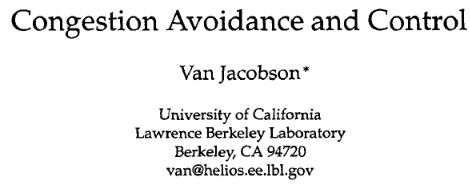
\includegraphics[width=0.6\textwidth]{../congest/jacobson-title}
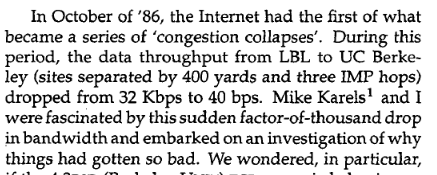
\includegraphics[width=0.6\textwidth]{../congest/jacobson-disaster}
\end{frame}

\begin{frame}<1>[label=jacobsonFixes]{fixes from Jacobson's 1987 paper}
\begin{tikzpicture}
\node[anchor=north west] (fixes) at (0, 0) {
    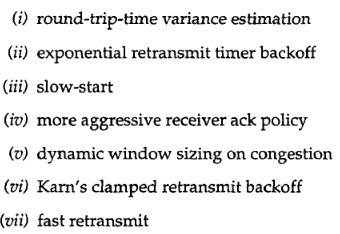
\includegraphics[width=0.6\textwidth]{../congest/jacobson-fixes}
};
%\path[draw,help lines] (0, 0) grid[step=1] (8, -5);
\begin{visibleenv}<2>
    \draw[red,ultra thick] (0, -3.8) rectangle (9, -4.4);
\end{visibleenv}
\begin{visibleenv}<4>
    \draw[red,ultra thick] (0, -2) rectangle (3, -2.8);
\end{visibleenv}
\begin{visibleenv}<3>
    \draw[red,ultra thick] (0, -5.4) rectangle (4.5, -6.2);
\end{visibleenv}
\end{tikzpicture}
\end{frame}

\begin{frame}[label=vegasrenotrace]{}
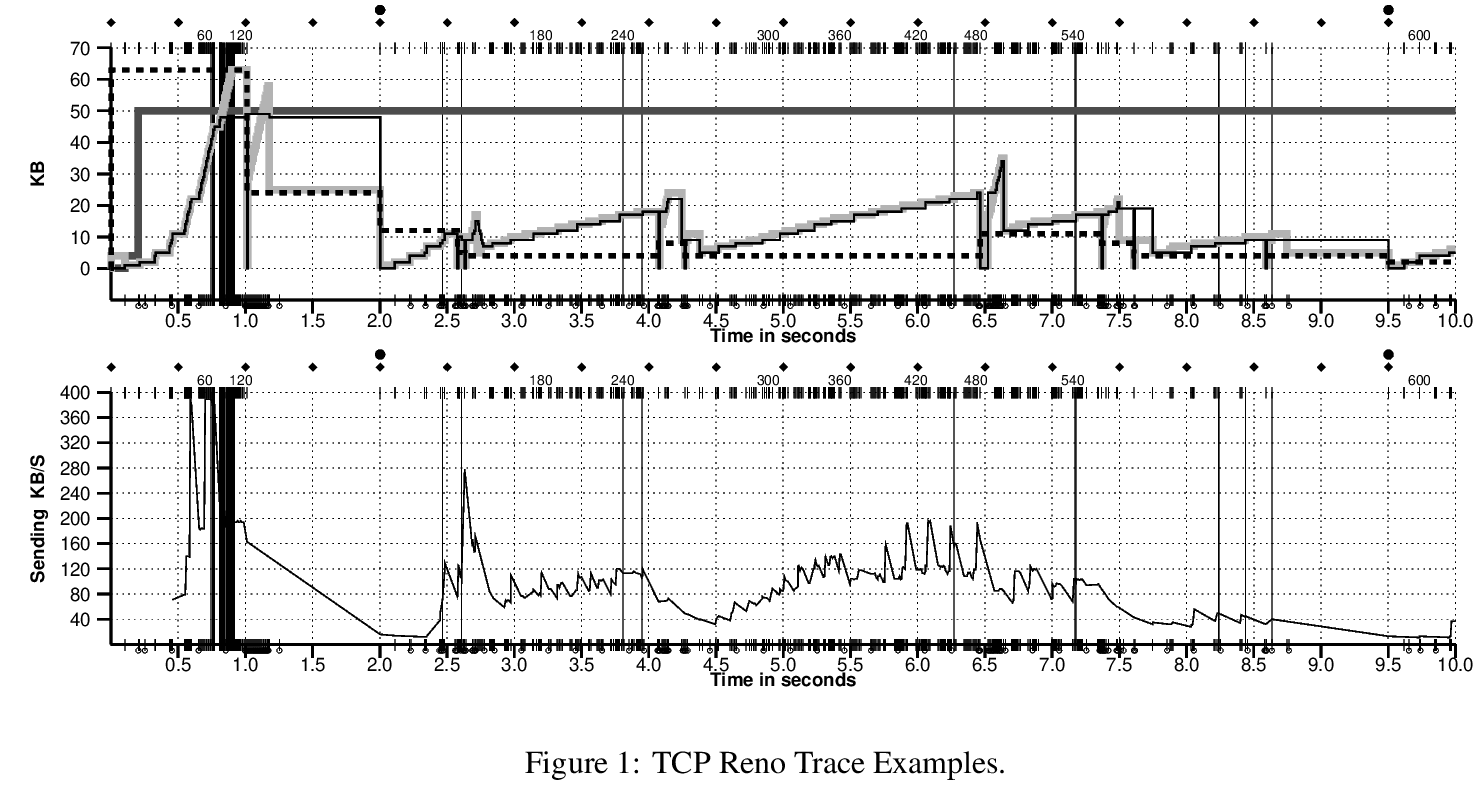
\includegraphics[width=0.9\textwidth]{../congest/vegas-fig1} \\
{
    \tiny from Brakmo, O'Malley, and Peterson, ``TCP Vegas: New techniques for
congestion detection and avoidance''} \\
    \small top thick, light-grey line = congestion window; dotted = slow start threshold
\end{frame}



\againframe<4>{jacobsonFixes}

\begin{frame}{``slow start''}
    \begin{itemize}
    \item not very well named
    \vspace{.5cm}
    \item problem is that additive increase doesn't find capacity quickly
    \item exponential(ish) increase to find \textit{initial} window size
    \end{itemize}
\end{frame}

\begin{frame}{``slow start'' on connection begin}
    \begin{itemize}
    \item set window size = 1 packet
    \item increase by one packet for each ACK
    \item \ldots until first packet loss
    \vspace{.5cm}
    \item then revert to additive increase
        \begin{itemize}
        \item actually slower at increasing
        \end{itemize}
    \end{itemize}
\end{frame}

\begin{frame}{``slow start'' later}
    \begin{itemize}
    \item keep track of window size after multiplicative decrease
    \item called \texttt{ssthresh}
        \begin{itemize}
        \item probably variable name in BSD code for this
        \end{itemize}
    \vspace{.5cm}
    \item on timeout (not dupack), reset window size to 1 packet, BUT
    \item use `slow start' until ssthresh reached or more congestion
        \begin{itemize}
        \item backoff network more aggressively, and
        \item hopefully find correct new window size faster?
        \end{itemize}
    \end{itemize}
\end{frame}
 % FIXME: picture

\subsection{exercise}
\begin{frame}{slow start effect}
    \begin{itemize}
    \item suppose we never leave slow start in connection between A and B and:
    \vspace{.5cm}
    \item A sends 4 packets to B
    \item after receiving 4 packets, B sends 8 packets to A
    \item after receiving those packets A sends 1 packet to B
    \vspace{.5cm}
    \item how many round-trip times does this take?
    \end{itemize}
\end{frame}


\subsection{some more graphs}
\againframe<2>{vegasrenotrace}
\begin{frame}{TCP `Tahoe' w/ one loss}
\tiny from Kevin Fall and Sally Floyd, ``Simulation-based Comparisons of Tahoe, Reno, and SACK TCP'' \\
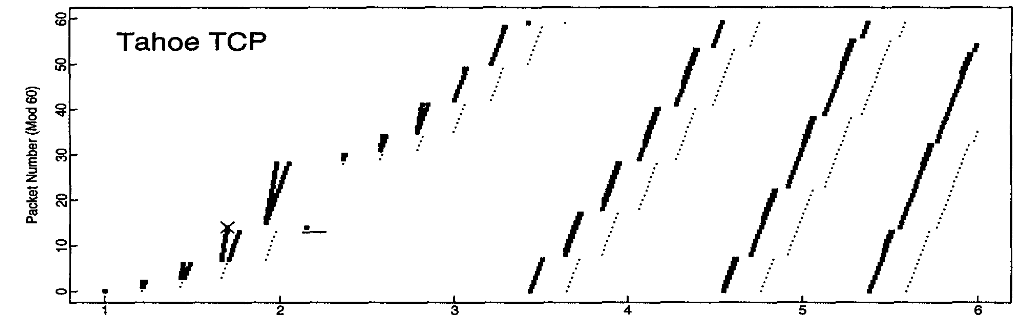
\includegraphics[width=\textwidth]{../congest/fall-floyd-fig2-tahoe} \\
TCP Tahoe = slow start, fast retransmit, no fast recovery 
\end{frame}

\begin{frame}{TCP `Reno' w/ one loss}
\tiny from Kevin Fall and Sally Floyd, ``Simulation-based Comparisons of Tahoe, Reno, and SACK TCP'' \\
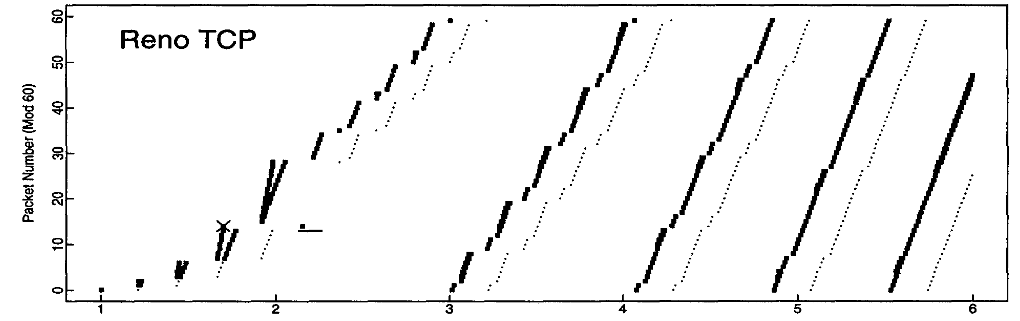
\includegraphics[width=\textwidth]{../congest/fall-floyd-fig2-reno}
TCP Reno = slow start, fast retransmit/recovery
\end{frame}


\section{missing piece: reverse path}
\begin{frame}{the reverse path}
    \begin{itemize}
    \item so far: assuming congestion on sender to receiver path
    \item but we can also have congestion in other direction
        \begin{itemize}
        \item network becomes overloaded with ACKs
        \end{itemize}
    \item hopefully rare because ACKs are small, but\ldots
    \item but worth some special mitigations
    \end{itemize}
\end{frame}

\begin{frame}{delayed ACKs}
\begin{itemize}
\item RFC 1122 {\small(Requirements for Internet Hosts --- Communication Layers)}
    \begin{itemize}
    \item ``A host that is receiving a stream of TCP data segments can increase efficiency\ldots by sending fewer than one ACK (acknowledgment) per data segment received; this is known as a ``delayed ACK''\ldots ''
    \end{itemize}
\item usually enabled these days
\item adds some latency, so Linux lets you disable on per-connection basis
\end{itemize}
\end{frame}


\section{aside: some queuing theory}
\begin{frame}{diversion: some queuing theory}
    \begin{itemize}
    \item queuing theory: applied probability
    \item talks about how queues work
    \vspace{.5cm}
    \item applies to networks and anything else with ``waiting in line''
    \end{itemize}
\end{frame}

\begin{frame}{queue measurements}
    \begin{itemize}
    \item arrival rate
    \item service time (amount of time after waiting in line)
    \item utilization = arrival rate / service time
    \vspace{.5cm}
    \item if single thing can be processed at a time, then max utilization = 100\%
        \begin{itemize}
        \item higher implies ``infinitely'' long queues
        \end{itemize}
    \end{itemize}
\end{frame}

\begin{frame}{M/M/1/$\infty$ queue}
    \begin{itemize}
    \item next slides: results for M/M/1/$\infty$ queue
    \vspace{.5cm}
    \item M (memoryless) --- random arrival (exponential dist.)
    \item M --- random service time (exponential dist.)
    \item 1 --- one ``server'' (thing that can process packets)
    \item $\infty$ --- unlimited queue length
    \end{itemize}
\end{frame}

\begin{frame}{M/M/1/$\infty$ queue length}
    \begin{itemize}
    \item mean queue length \[\frac{\text{arrival rate}}{\text{service rate} - \text{arrival rate}}\]
    \end{itemize}
\begin{tikzpicture}
\begin{axis}[width=12cm,height=5cm,xlabel=arrival rate (portion of service rate),ylabel=queue length,xmin=0,xmax=1.2,ymin=0,ymax=10]
\addplot[blue,ultra thick,domain=0:1,samples=128]{x/(1-x)};
\end{axis}
\end{tikzpicture}
    \begin{itemize}
    \item<2-> practical implication: \myemph{need to run networks at much less than full utilization}
    \end{itemize}
\end{frame}

\begin{frame}{M/M/1/$\infty$ queue length std. deviation}
    \begin{itemize}
    \item \[\sqrt{\frac{\text{utilization}}{\left(1 - \text{utilization}\right)^2}}\]
    \end{itemize}
\begin{tikzpicture}
\begin{axis}[width=12cm,height=6cm,xlabel=arrival rate (portion of service rate),ylabel=queue length,xmin=0,xmax=1,ymin=0,ymax=10]
\addplot[blue,ultra thick,domain=0:1,samples=128]{sqrt(x/(1-x)^2)};
\end{axis}
\end{tikzpicture}
\end{frame}

\begin{frame}{approx 95th pctile v mean queue length}
\begin{tikzpicture}
\begin{axis}[width=12cm,height=8cm,xlabel=arrival rate (portion of service rate),ylabel=queue length,xmin=0,xmax=1,ymin=0,ymax=10]
\addplot[blue,ultra thick,domain=0:1,samples=128]{x/(1-x)+1.96*sqrt(x/(1-x)^2)};
\addplot[dotted,ultra thick,violet,domain=0:1,samples=128]{x/(1-x)};
\end{axis}
\end{tikzpicture}
\end{frame}


\section{deep queues?}
\usetikzlibrary{arrows.meta}
\begin{frame}{filling buffers}
\begin{tikzpicture}
\tikzset{
    axis/.style={
        draw,ultra thick,-Latex
    },
    normal mark/.style={
        fill=black,
        alt=<5->{fill=black!50},
    },
    normal adjust/.style={
        line width=.5mm,draw=black!50!red,-Latex,
        alt=<5->{draw=black!50!red!50},
    },
}
\begin{scope}[x=1.2cm,y=1.2cm] 
    \path[fill=red!10] (5.5, 0) -- (5.0, 0) -- (0, 5) -- (0, 5.5) -- (5.5, 5.5) -- cycle;
    \path[axis] (0, 0) -- (5.5, 0)
        node[midway,below] {flow 1 bandwidth};
    \path[axis] (0, 0) -- (0, 5.5)
        node[midway,left,align=right] {flow 2\\bandwidth};
    \path[draw,dashed,very thick] (5, 0) -- (0, 5);
    \node[text=red] at (4, 4) {
        overloaded
    };
    \node[text=black,rotate=-45] at (2.25, 2.25) {
        buffers almost full
    };
    \path[draw,dotted,very thick] (4, 0) -- (0, 4);
\end{scope}
\end{tikzpicture}
\end{frame}

\begin{frame}{big buffers? (in 2011 or so)}
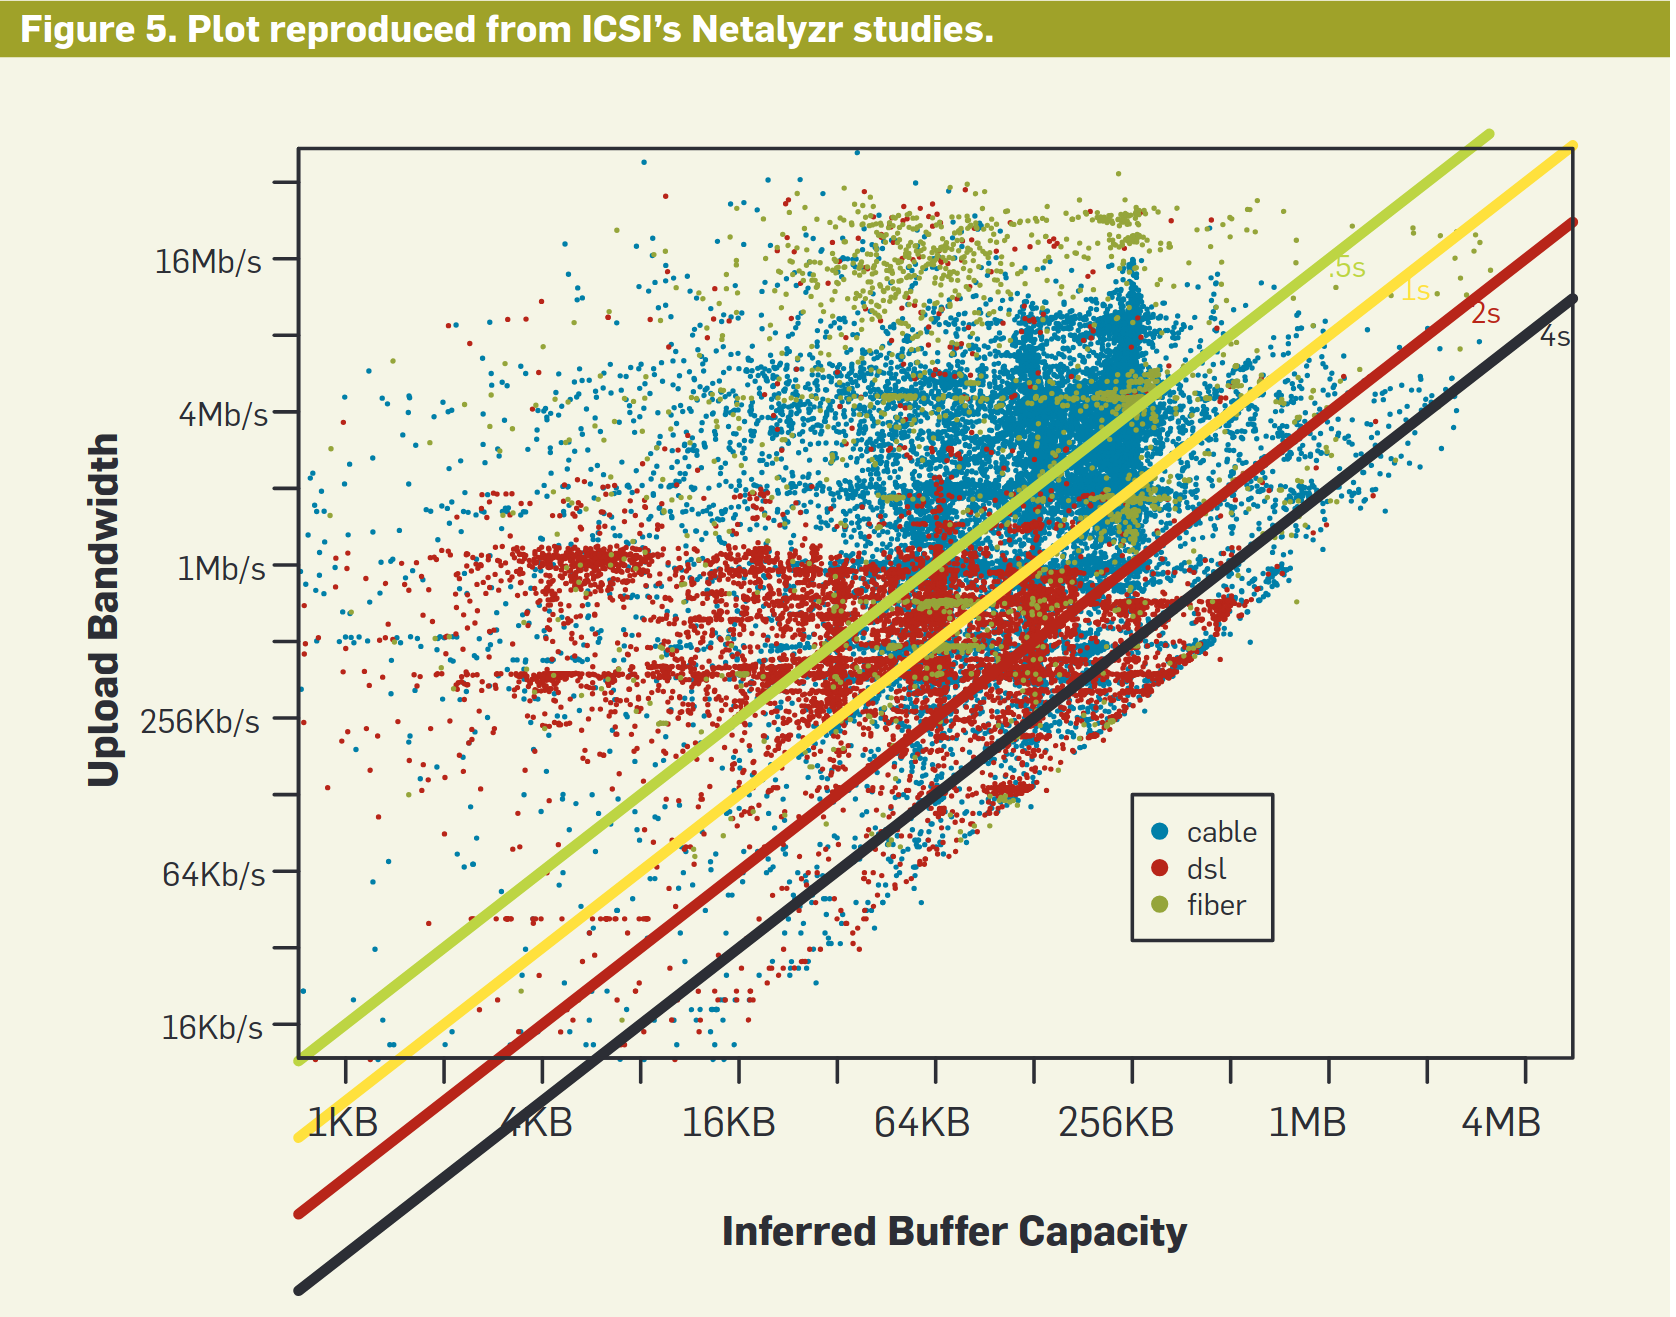
\includegraphics[width=0.6\textwidth]{../congest/cacm-bufferbloat-fig5}

{\scriptsize Jim Gettys and Kathleen Nichols, \\ ``Bufferbloat: Dark Buffers in the Internet'' (CACM, Jan 2012)}
\end{frame}

\begin{frame}{problems with big buffers}
    \begin{itemize}
    \item high latency --- bad for some applications
    \item slower response to congestion
        \begin{itemize}
        \item 1 second round trip time = 1 second to detect congestion
        \item more likely to have `congestion collapse'
        \end{itemize}
    \end{itemize}
\end{frame}

\begin{frame}{avoiding big buffers}
    \begin{itemize}
    \item multiple fixes (that can be combined):
    \vspace{.5cm}
    \item use smaller buffers?
        \begin{itemize}
        \item simpliest solution
        \end{itemize}
    \item detect congestion without full buffer\ldots
        \begin{itemize}
        \item \myemph<3>{by choosing when/which packets to drop better?}
        \item \myemph<4>{by using something other than drops?}
        \end{itemize}
    \end{itemize}
\end{frame}


\section{missing Jacobson pieces}

\subsection{variance estimation}
\againframe<5>{jacobsonFixes}
\begin{frame}{timeout setting}
    \begin{itemize}
    \item goal in setting timeouts:
        \begin{itemize}
        \item timeout triggering almost always means dropped packet
        \end{itemize}
    \item to do this want \textit{highest likely round trip time}
    \vspace{.5cm}
    \item original TCP heuristic: twice RTT estimate
    \end{itemize}
\end{frame}

\begin{frame}{RTT variation exercise (1)}
    \begin{itemize}
    \item let's say 1 ms tranmission delay + 20 ms propogation delay
    \item and queue depth ranges `randomly' from 1 to 10
    \item exercise: round-trip-time?
        \begin{itemize}
        \item<2-> 42 ms with no queue
        \item<2-> +1 ms per queue depth
        \item<2-> 43 to 52 ms
        \end{itemize}
    \end{itemize}
\end{frame}

\begin{frame}{RTT variation exercise (2)}
    \begin{itemize}
    \item let's say 1 ms tranmission delay + 10 ms propogation delay
    \item and queue depth ranges `randomly' from 10 to 40
    \item exercise: round-trip-time?
        \begin{itemize}
        \item<2-> 12 ms with no queue
        \item<2-> +1 ms per queue depth
        \item<2-> 22 to 52 ms
        \end{itemize}
    \end{itemize}
\end{frame}

\begin{frame}{how does original timeout do?}
    \begin{itemize}
    \item works well when queuing delay small relative to other delays
    \item works poorly when queuing delay high
    \item \ldots because queuing delay won't be consistent!
    \end{itemize}
\end{frame}

\begin{frame}{new timeout formula}
    \begin{itemize}
    \item estimate mean deviation of RTT (= difference from average)
    \item similar exponentially weighted moving average
    \vspace{.5cm}
    \item timeout = RTT estimate + 2 $\times$ RTT deviation estimate
    \end{itemize}
\end{frame}



\subsection{exponential backoff}
\againframe<6>{jacobsonFixes}
\begin{frame}{normal backoff}
    \begin{itemize}
    \item problem: what if we have multiple timeouts
    \vspace{.5cm}
    \item let's say timeout is 1 time unit
    \item transmit at 1 time unit, 2 time units, 3 time units, 4 time units, etc.
    \vspace{.5cm}
    \item problem: if the network is overloaded \textit{from retransmissions} won't stop it
        \begin{itemize}
        \item \ldots but window size reduction should make number of packets retransmitted \textit{per connection} low
        \item (so probably not so important with corrected window size management?)
        \end{itemize}
    \end{itemize}
\end{frame}

\begin{frame}{exponential backoff}
    \begin{itemize}
    \item instead of: \\
    \item transmit at 1 time unit, 2 time units, 3 time units, 4 time units, etc.
    \vspace{.5cm}
    \item do something like: \\
    transmit at 1 time unit, 3 time units, 7 time units, 15 time units, etc.
    \end{itemize}
\end{frame}

\begin{frame}{exponential backoff theory}
    \begin{itemize}
    \item for binary exponential backoff 
        \begin{itemize}
        \item timeout for $i$th retransmission is $2^i \times \text{base timeout}$
        \end{itemize}
    \item intuition: avoids overloading network by being a lot less aggressive
        \begin{itemize}
        \item what you `should' do for repeated timeouts due to congestion
        \end{itemize}
    \item not aware of good theoretical results in TCP context
        \begin{itemize}
        \item famous result that this type of backoff is good for things like deciding when to retransmit on shared wired/wireless medium
        \item (Goodman et al, ``On Stability of Ethernet'')
        \end{itemize}
    \end{itemize}
\end{frame}


\section{TCP variants}
\begin{frame}{``traditional'' TCP variant names}
\begin{itemize}
\item everything we've talked about as standard = NewReno
\vspace{.5cm}
\item Tahoe --- slow start + redo slow start on any loss + fast retransmit
\item Reno --- Tahoe + halve window size on dup ACKs
\item NewReno --- Reno + fast recovery (send extra during fast retransmit)
\item SACK --- NewReno + use selective acknowledgments
\end{itemize}
\end{frame}

\begin{frame}{more recent TCP variants}
\begin{itemize}
\item BIC, CUBIC --- loss-based schemes that vary increase/decrease algorithm
\item Vegas, BBR, FAST, Compound, Westwood --- schemes that use latency/bandwidth to detect congestion
    \begin{itemize}
    \item (later topic)
    \end{itemize}
\item (and there are many, many more)
\end{itemize}
\end{frame}




\section{congestion missing pieces}
\begin{frame}{some connected questions}
    \begin{itemize}
    \item do we really need packet loss?
    \item what does congestoin control due to latency?
    \end{itemize}
\end{frame}

\section{other congestion signals}

\begin{frame}{other congestion signals}
\begin{itemize}
\item so far: detecting congestion via drops
    \begin{itemize}
    \item need data to go missing
    \item transmitting redundant data
    \item filling up buffers causing high latency
    \end{itemize}
\vspace{.5cm}
\item some alternate ideas:
\item have switches/routers `mark' packets
\item latency from longer queues
\end{itemize}
\end{frame}


\subsection{explicit congestion notification}

\againframe<2>{otherSig}
\begin{frame}{ECN}
\begin{itemize}
\item explicit congestion notification
\vspace{.5cm}
\item when buffer `close' to full
\item switches/router set `ECN' bit in some packets
    \begin{itemize}
    \item field in IP header
    \end{itemize}
\item ECN bit echoed back in ACKs
\end{itemize}
\end{frame}

\begin{frame}{ECN timeline}
\begin{tikzpicture}
\tikzset{
    box/.style={thick},
    message/.style={draw,thick,-Latex},
    failure/.style={draw,ultra thick,red,cross out,minimum width=1cm,minimum height=1cm},
    every node/.style={inner sep=0.1mm},
}
\begin{scope}[xshift=1cm,x=0.9cm]
\draw[box] (0, 0) rectangle ++(2, -6) 
    node[midway,align=center] {machine\\A};
\draw[box] (5, 0) rectangle ++(2, -6) 
    node[midway,align=center] {switch};
\draw[box] (13, 0) rectangle ++(2, -6) 
    node[midway,align=center] {machine\\B};
\draw[message] (2, -0.5) -- (13, -1.5) node[pos=0.25,above,sloped] {[no ECN]{0}: ``The ''}
    node[pos=0.75,above,sloped] {[no ECN]{0}: ``The ''};
\draw[message] (13, -1.75) -- (2, -2.75) node[pos=0.25,sloped,below] {got up to {0}};
\draw[message] (2, -1) -- (13, -2) node[pos=0.25, above, sloped] {[no ECN]{1}: ``meeting''}
    node[pos=0.75,above,sloped] {\myemph{[yes ECN]}{0}: ``The ''};
\draw[message] (13, -2.25) -- (2, -3.25) node[pos=0.25, sloped,below] {got up to {1} \myemph{WITH ECN mark}};

% in response to got 0
\draw[message] (2, -3) -- (13, -4) node[pos=0.5, above, sloped] {[no ECN] {2}: `` is at ''};
\draw[message] (13, -4.25) -- (2, -5.25) node[pos=0.25, sloped,below] {got up to {2}};
% in response to got 1
\draw[message] (2, -3.5) -- (13, -4.5) node[pos=0.5, above, sloped] {[no ECN] {3}: ``12pm.''};
\draw[message] (13, -4.75) -- (2, -5.75) node[pos=0.25, sloped,below] {got up to {3}};
\end{scope}
\end{tikzpicture}
\begin{itemize}
\item data sent has place for ECN bit to be placed
\item switch modifies ECN bit \myemph{if buffer close to full}
\item ACK indicates if ECN bit was set
\end{itemize}
\end{frame}



\subsection{watching latency, etc.}

\againframe<3>{otherSig}
\begin{frame}{very different congestion control}
    \begin{itemize}
    % FIXME: Fig 32 from TCPCC book
    \item fuller queues $\rightarrow$ higher latency
    \item fuller queues $\rightarrow$ throughput same as window increases
    \vspace{.5cm}
    \item<2-> strategy: monitor throughput/latency to detect full queues
        \begin{itemize}
        \item goal: fill link without making queue grow in size
        \item react before dropped packets happen
        \end{itemize}
    \end{itemize}
\end{frame}

\begin{frame}{`Vegas'-style congestion control}
    \begin{itemize}
    \item record ``base'' round-trip time
        \begin{itemize}
        \item connection start or lowest observed
        \end{itemize}
    \item ``ideal'' throughput should be one window / base round trip time
        \begin{itemize}
        \item (Vegas paper calls this ``expected'' throughput)
        \item what would happen with no queuing delay
        \end{itemize}
    \vspace{.5cm}
    \item goal: control what ``ideal'' - actual throughput is
        \begin{itemize}
        \item if 0, queues are probably empty, can increase window
        \item if large, queues are too big, decrease window
        \end{itemize}
    \end{itemize}
\end{frame}

\begin{frame}{BBR-style congestion control}
    \begin{itemize}
    \item \myemph<2>{if queues are empty}, larger window:
    \item latency stays the same and throughput increases
    \vspace{.5cm}
    \item \myemph<3>{if queues are filling}, larger window:
    \item throughput stays the same and latency increases
    \vspace{.5cm}
    \item<4-> observe effect of sending more/fewer packets periodically
    \item<4-> estimate `boundary' based on observed latency/throughput
    \item<4-> keep window size near boundary most of the time
    \end{itemize}
\end{frame}



\section{drop-tail and some of its problems}

\usetikzlibrary{arrows.meta,patterns}

\begin{frame}{FIFO + drop-tail}
    \begin{itemize}
    \item \myemph<2-4>{scheduling policy: first-in first-out (FIFO)}
    \item \myemph<5>{drop policy: drop tail}
    \end{itemize}
\begin{tikzpicture}
    \draw[thick] (0, -.5) rectangle (8, .5);
    \begin{visibleenv}<2>
        \path[draw,Latex-,line width=1mm] (0.5, -.5) -- ++(0, -2) node[below] {newest message};
        \path[draw,Latex-,line width=1mm] (7.5, -.5) -- ++(0, -2) node[below] {next out / oldest message};
    \end{visibleenv}
    \begin{visibleenv}<3>
        \path[fill=red!30,pattern=north west lines,pattern color=black] (7, -.5) rectangle ++(1, 1);    
        \path[draw,Latex-,line width=1mm] (7.5, -.5) -- ++(0, -2) node[below] {empty? first message placed here};
    \end{visibleenv}
    \begin{visibleenv}<4>
        \path[fill=violet!30] (5, -.5) rectangle ++(3, 1);    
        \path[fill=red!30,pattern=north west lines,pattern color=black] (4, -.5) rectangle ++(1, 1);    
        \path[draw,Latex-,line width=1mm] (4.5, -.5) -- ++(0, -2) node[below] {partly full? use next slot};
    \end{visibleenv}
    \begin{visibleenv}<5>
        \path[fill=violet!30] (0, -.5) rectangle ++(8, 1);
    \end{visibleenv}
    \foreach \x in {1,2,3,4,5,6,7} {
        \draw (\x, -.5) -- (\x, .5);
    }
    \draw[ultra thick,Latex-] (0, 0) -- ++(-2, 0);
    \draw[alt=<4>{draw=red,text=red},ultra thick,dotted,-Latex] (-.9, 0) to[in=90,out=0] ++(.5,-1) node[below] 
        (discarded text) {discarded};
    \begin{visibleenv}<5>
        \node[anchor=north] at (discarded text.south) {full? discard new packets};
    \end{visibleenv}
    \draw[ultra thick,-Latex] (8, 0) -- ++(2, 0);
    \node[anchor=south] at (.5, .5) {tail};
    \node[anchor=south] at (7.5, .5) {head};
    \begin{visibleenv}<3-5>
        \path[draw,black!50,very thick,dashed,pattern=north west lines, pattern color=black!50]
            (-2.5, -.5) rectangle ++(1, 1);
    \end{visibleenv}
\end{tikzpicture}
\end{frame}




\section{priority queuing}

\usetikzlibrary{arrows.meta,patterns,shapes.misc}

\begin{frame}{priority queue}
    \begin{itemize}
    \item assign priorities to flows
    \item drop packet from lowest priority flow possible
    \item on ties, choose other drop strategy
    \end{itemize}
\end{frame}

\begin{frame}{priority-based dequeue}
\begin{tikzpicture}
\tikzset{
    first flow/.style={pattern=checkerboard,pattern color=blue!30},
    second flow/.style={fill=violet!30},
    ghost/.style={dashed,fill opacity=0.5},
    packet move line/.style={draw,line width=0.8mm},
}
    \begin{scope}[yshift=0cm]
        \foreach \x in {0,1,4,6,7} {
            \path[first flow] (\x, -.5) rectangle ++(1, 1);
        }
        \foreach \x in {2,3,5,8} {
            \path[second flow] (\x, -.5) rectangle ++(1, 1);
        }
        \draw[thick] (0, -.5) rectangle (9, .5);
        \foreach \x in {0,1,2,3,4,5,6,7,8} {
            \draw (\x, -.5) -- (\x, .5);
        }
        \draw[ultra thick] (8, -.5) rectangle ++(1,1);
        \path[packet move line,-{Latex[length=3mm]}] (9, 0) -- ++(1.5, 0);
    \end{scope}

    \begin{scope}[yshift=-2cm]
        \foreach \x in {0,1,3,7,8} {
            \path[first flow] (\x, -.5) rectangle ++(1, 1);
        }
        \foreach \x in {2,4,5,6} {
            \path[second flow] (\x, -.5) rectangle ++(1, 1);
        }
        \draw[thick] (0, -.5) rectangle (9, .5);
        \foreach \x in {0,1,2,3,4,5,6,7,8} {
            \draw (\x, -.5) -- (\x, .5);
        }
        \draw[ultra thick] (6, -.5) rectangle ++(1,1);
        \path[packet move line,-{Latex[length=3mm]}] (6.5, -.5) to[out=-90,in=180] ++(.5, -.5)
            -- ++(2, 0) to[out=0,in=-90] ++(.5, .5) to[in=180,out=90] ++(1, .5);
    \end{scope}
    
    \begin{scope}[yshift=-4cm]
        \foreach \x in {0,1,2,3,4,5,6,7,8} {
            \path[first flow] (\x, -.5) rectangle ++(1, 1);
        }
        \foreach \x in {} {
            \path[second flow] (\x, -.5) rectangle ++(1, 1);
        }
        \draw[thick] (0, -.5) rectangle (9, .5);
        \foreach \x in {0,1,2,3,4,5,6,7,8} {
            \draw (\x, -.5) -- (\x, .5);
        }
        \draw[ultra thick] (8, -.5) rectangle ++(1,1);
        \path[packet move line,-{Latex[length=3mm]}] (9, 0) -- ++(1.5, 0);
    \end{scope}
\end{tikzpicture}
\end{frame}

\begin{frame}{priority-based dropping}
\begin{tikzpicture}
\tikzset{
    first flow/.style={pattern=checkerboard,pattern color=blue!30},
    second flow/.style={fill=violet!30},
    ghost/.style={dashed,fill opacity=0.5},
    packet move line/.style={draw,line width=0.8mm},
}
    \begin{scope}[yshift=-2cm]
        \foreach \x in {0} {
            \draw (\x, -1) rectangle ++(1,1);
            \draw (\x, 0) rectangle ++(1,1);
            \path[first flow,ghost] (\x, -1) rectangle ++(1, 1);
            \node[cross out,draw=red,line width=1mm,minimum width=1cm,minimum height=1cm] at (\x+.5, -.5) {};
            \path[second flow,ghost] (\x, 0) rectangle ++(1, 1);
        }
        \foreach \x in {1,4,6,7,8} {
            \path[first flow] (\x, -.5) rectangle ++(1, 1);
        }
        \foreach \x in {-3,2,3,5} {
            \path[second flow] (\x, -.5) rectangle ++(1, 1);
        }
        \foreach \x in {1,2,3,4,5,6,7,8} {
            \draw (\x, -.5) -- (\x, .5);
        }
        \path[draw] (1, -.5) rectangle (9, .5);
        \path[draw] (-3, -.5) rectangle (-2, .5);
        \path[packet move line,-{Latex[length=3mm]}] (-2, 0) -- (-1.5, 0) to[in=270,out=0]
            (-1., .25) to[in=180,out=90] (-0.75, .5) -- (0, .5);
        \path[packet move line,dotted,-{Latex[length=3mm]}] (.5,-1) -- ++(0, -.5cm);% node[below=-2mm] {discarded};
    \end{scope}
    \begin{scope}[yshift=-4.5cm]
        \foreach \x in {-1.5} {
            \path[first flow,ghost] (\x, -.7) rectangle ++(1, 1);
            \node[cross out,draw=red,line width=1mm,minimum width=1cm,minimum height=1cm] at (\x+.5, -.2) {};
        }
        \foreach \x in {-3,0,1,4,6,7,8} {
            \path[first flow] (\x, -.5) rectangle ++(1, 1);
        }
        \foreach \x in {2,3,5} {
            \path[second flow] (\x, -.5) rectangle ++(1, 1);
        }
        \foreach \x in {1,2,3,4,5,6,7,8} {
            \draw (\x, -.5) -- (\x, .5);
        }
        \path[draw] (0, -.5) rectangle (9, .5);
        \path[draw] (-3, -.5) rectangle (-2, .5);
        \path[packet move line,-{Latex[length=3mm]}] (-2, 0) -- (-2.0, 0) to[in=270,out=0] (-1.75, 0.25) -- (-1.75, .5) to[in=180,out=90] (-1.5, 0.75)
           -- (-1.25, 0.75) to[out=0,in=45+90-45] (-1, .5) -- (-1, -.2+.5);
        \path[packet move line,dotted,-{Latex[length=3mm]}] (-1,-.7) -- ++(0, -.5cm);% node[below=-2mm] {discarded};
    \end{scope}
    \begin{scope}[yshift=-7cm]
        \foreach \x in {-1.5} {
            \path[second flow,ghost] (\x, -.7) rectangle ++(1, 1);
            \node[cross out,draw=red,line width=1mm,minimum width=1cm,minimum height=1cm] at (\x+.5, -.2) {};
        }
        \foreach \x in {-3,0,1,2,3,4,5,6,7,8} {
            \path[second flow] (\x, -.5) rectangle ++(1, 1);
        }
        \foreach \x in {1,2,3,4,5,6,7,8} {
            \draw (\x, -.5) -- (\x, .5);
        }
        \path[draw] (0, -.5) rectangle (9, .5);
        \path[draw] (-3, -.5) rectangle (-2, .5);
        \path[packet move line,-{Latex[length=3mm]}] (-2, 0) -- (-2.0, 0) to[in=270,out=0] (-1.75, 0.25) -- (-1.75, .5) to[in=180,out=90] (-1.5, 0.75)
           -- (-1.25, 0.75) to[out=0,in=45+90-45] (-1, .5) -- (-1, -.2+.5);
        \path[packet move line,dotted,-{Latex[length=3mm]}] (-1,-.7) -- ++(0, -.5cm);% node[below=-2mm] {discarded};
    \end{scope}
\end{tikzpicture}
\end{frame}

\begin{frame}{priority-based dropping (alt)}
\begin{tikzpicture}
\tikzset{
    first flow/.style={pattern=checkerboard,pattern color=blue!30},
    second flow/.style={fill=violet!30},
    ghost/.style={dashed,fill opacity=0.5},
    packet move line/.style={draw,line width=0.8mm},
}
    \begin{scope}[yshift=-2cm]
        \foreach \x in {-1} {
            \path[first flow,ghost] (\x, -.7) rectangle ++(1, 1);
            \node[cross out,draw=red,line width=1mm,minimum width=1cm,minimum height=1cm] at (\x+.5, -.2) {};
        }
        \foreach \x in {0,1,2,3,4} {
            \path[first flow] (\x, -.5) rectangle ++(1, 1);
        }
        \foreach \x in {5.5} {
            \path[second flow,ghost] (\x, -.3) rectangle ++(1, 1);
        }
        \foreach \x in {-4,6.5,7.5} {
            \path[second flow] (\x, -.5) rectangle ++(1, 1);
        }
        \path[draw,thick] (-4, -.5) rectangle (-3, .5);
        \draw[thick] (0, -.5) rectangle (5, .5);
        \draw[thick] (5.5, -.3) rectangle ++(1, 1);
        \draw[thick] (-1, -.7) rectangle ++(1, 1);
        \draw[thick] (6.5, -.5) rectangle (8.5, .5);
        \foreach \x in {0,1,2,3,4,6.5,7.5,8.5} {
            \draw (\x, -.5) -- (\x, .5);
        }
        \path[packet move line,-{Latex[length=3mm]}] (-3, 0) -- (-2.0, 0) to[in=270,out=0] (-1.5, 0.5) to[in=180,out=90] (-.5, 1.2)
           -- (4.5, 1.2) to[out=0,in=45+90-45] (6, 0.7);
        \path[packet move line,dotted,-{Latex[length=3mm]}] (-.5,-.7) -- ++(0, -.5cm);% node[below=-2mm] {discarded};
    \end{scope}
    \begin{scope}[yshift=-4.5cm]
        \foreach \x in {-1.5} {
            \path[first flow,ghost] (\x, -.7) rectangle ++(1, 1);
            \node[cross out,draw=red,line width=1mm,minimum width=1cm,minimum height=1cm] at (\x+.5, -.2) {};
        }
        \foreach \x in {-4,0,1,2,3,4} {
            \path[first flow] (\x, -.5) rectangle ++(1, 1);
        }
        \foreach \x in {5.5,6.5,7.5} {
            \path[second flow] (\x, -.5) rectangle ++(1, 1);
        }
        \path[draw,thick] (-4, -.5) rectangle (-3, .5);
        \draw[thick] (0, -.5) rectangle (5, .5);
        \draw[thick] (5.5, -.5) rectangle ++(1, 1);
        \draw[thick] (-1.5, -.7) rectangle ++(1, 1);
        \draw[thick] (6.5, -.5) rectangle (8.5, .5);
        \foreach \x in {0,1,2,3,4,6.5,7.5,8.5} {
            \draw (\x, -.5) -- (\x, .5);
        }
        \path[packet move line,-{Latex[length=3mm]}] (-3, 0) -- (-3.0, 0) to[in=270,out=0] (-2.5, 0.5) to[in=180,out=90] (-2, 1)
           -- (-1.5, 1) to[out=0,in=45+90-45] (-1, -.2+.5);
        \path[packet move line,dotted,-{Latex[length=3mm]}] (-1,-.7) -- ++(0, -.5cm);% node[below=-2mm] {discarded};
    \end{scope}
    \begin{scope}[yshift=-7cm]
        \foreach \x in {-1.5} {
            \path[second flow,ghost] (\x, -.7) rectangle ++(1, 1);
            \node[cross out,draw=red,line width=1mm,minimum width=1cm,minimum height=1cm] at (\x+.5, -.2) {};
        }
        \foreach \x in {-4,0,1,2,3,4} {
            \path[second flow] (\x, -.5) rectangle ++(1, 1);
        }
        \foreach \x in {5,6,7} {
            \path[second flow] (\x, -.5) rectangle ++(1, 1);
        }
        \path[draw,thick] (-4, -.5) rectangle (-3, .5);
        \draw[thick] (0, -.5) rectangle (5, .5);
        \draw[thick] (5, -.5) rectangle ++(1, 1);
        \draw[thick] (-1.5, -.7) rectangle ++(1, 1);
        \draw[thick] (6, -.5) rectangle (8, .5);
        \foreach \x in {0,1,2,3,4,6,7,8} {
            \draw (\x, -.5) -- (\x, .5);
        }
        \path[packet move line,-{Latex[length=3mm]}] (-3, 0) -- (-3.0, 0) to[in=270,out=0] (-2.5, 0.5) to[in=180,out=90] (-2, 1)
           -- (-1.5, 1) to[out=0,in=45+90-45] (-1, -.2+.5);
        \path[packet move line,dotted,-{Latex[length=3mm]}] (-1,-.7) -- ++(0, -.5cm); % node[below=-2mm] {discarded};
    \end{scope}
\end{tikzpicture}
\end{frame}

\begin{frame}{priority: all or nothing}
    \begin{itemize}
    \item if flow A has greater priority than flow B
    \item and both can use full available bandwidth
    \vspace{.5cm}
    \item flow A gets full available bandwidth
    \item flow B gets no bandwidth (everything dropped)
    \end{itemize}
\end{frame}



\section{simple fair queuing}
% FIXME:
    % with packet arrivals synchornized to packet ends
    % what if arrives-in-middle
    % simultaing bit-by-bit sending

\section{weighted fair queuing}
\begin{frame}{weights instead of priorities}
    \begin{itemize}
    \item alternate idea: weights
    \item if flow A has weight 9, flow B has weight 1
    \item and both can use full availabile bandwidth
    \vspace{.5cm}
    \item flow A gets 90\% of bandwidth
    \item flow B gets 10\% of bandwidth
    \end{itemize}
\end{frame}




\section{backup slides}
\begin{frame}{backup slides}
\end{frame}


\section{recall: window size versus bandwidth}
\usetikzlibrary{arrows.meta,calc}

\begin{frame}[fragile,label=throughAndWindow]{throughput and window size}
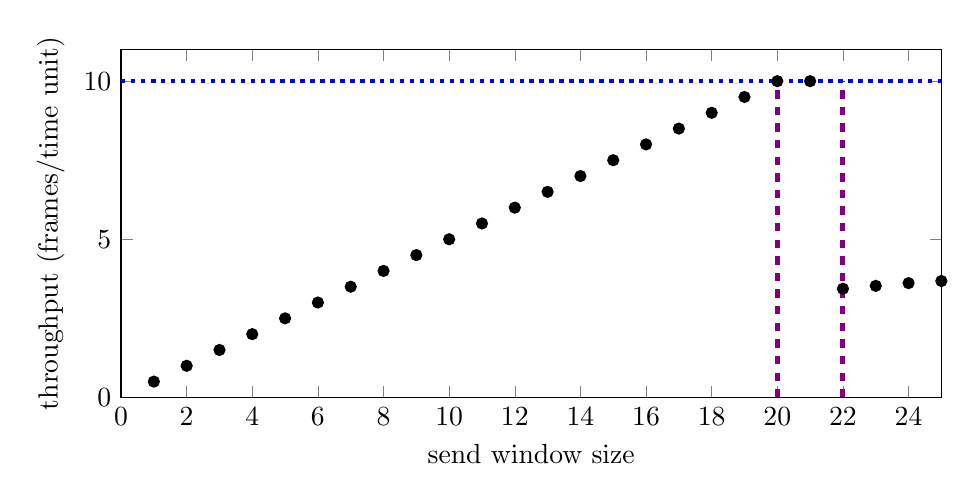
\begin{tikzpicture}
\begin{axis}[width=12cm,height=6cm,
    xlabel=send window size,
    ylabel=throughput (frames/time unit),
    xmin=0,xmax=25,ymin=0]
\addplot[only marks] coordinates {
(1, 0.5000025000125)
(2, 1.0000090000810007)
(3, 1.4999925000374998)
(4, 2.0000280003920055)
(5, 2.500037500562508)
(6, 3.000003000003)
(7, 3.5000035000035)
(8, 4.000048000576006)
(9, 4.499842505512307)
(10, 5.000025000125)
(11, 5.499975250111374)
(12, 5.99977200866367)
(13, 6.499710762871052)
(14, 6.999811005102861)
(15, 7.4996812635462975)
(16, 7.999680012799485)
(17, 8.499426288725509)
(18, 8.999361045365776)
(19, 9.499202067026369)
(20, 9.999100080971061)
(21, 9.999100080973866)
(22, 3.435635094325549)
(23, 3.5274986154570636)
(24, 3.613708966335035)
(25, 3.6808686850100703)
(26, 3.753260645186032)
(27, 3.8487443471573166)
(28, 3.925956461143474)
};
\addplot[blue,dotted,ultra thick,domain=0:25] {10};
    \draw[violet,dashed,ultra thick] (axis cs:20,0) -- (axis cs:20, 10)
     coordinate (empty queue mark);
    \draw[violet,dashed,ultra thick] (axis cs:21.99,0) -- (axis cs:21.99, 10)
     coordinate (full queue mark);
\end{axis}
\end{tikzpicture}
\end{frame}

\usetikzlibrary{arrows.meta,calc}

\begin{frame}{simple network model}
\begin{tikzpicture}
\draw[ultra thick,arrows={-Latex}] (0, 0) node[left] {sender} -- (1, 0);
\draw[thick] (1, -.5) rectangle (3, .5);
\foreach \x in {2,2.2,2.4,2.6,2.8} {
    \draw (\x, -.5) -- (\x, .5);
}
\node[anchor=south,align=center] at (2, .5) {
    loss when full
};
\node[anchor=north,align=center] at (2, -.5) (queue label) {
    queue
};
\node[anchor=north,font=\small] at ([yshift=.2cm]queue label.south) {
    capacity 20
};
\draw[ultra thick,arrows={-Latex}] (3, 0) -- (10, 0) node[right]{receiver}
    node[midway,fill=white,draw=black,very thick,align=left] {
        10 data frames/time unit \\
        1 time unit delay
    };
\begin{scope}[shift={(10, -3)},x=-1cm]
    \draw[ultra thick,arrows={-Latex}] (0, 0) node[right] {receiver} -- (1, 0);
    \draw[thick] (1, -.5) rectangle (3, .5);
    \foreach \x in {2,2.2,2.4,2.6,2.8} {
        \draw (\x, -.5) -- (\x, .5);
    }
    \node[anchor=south,align=center] at (2, .5) {
        loss when full
    };
    \node[anchor=north,align=center] at (2, -.5) (queue label) {
        queue
    };
    \node[anchor=north,font=\small] at ([yshift=.2cm]queue label.south) {
        capacity 20
    };
    \draw[ultra thick,arrows={-Latex}] (3, 0) -- (10, 0) node[left]{sender}
        node[midway,fill=white,draw=black,very thick,align=left] {
            100 ACK frames/time unit \\
            1 time unit delay
        };
\end{scope}
\end{tikzpicture}
\begin{itemize}
\item simulator from upcoming assignment
    \begin{itemize}
    \item command line \texttt{--delay 1 --bandwidth-forward 10 --bandwidth-backward 100 --buffer 30}
    \end{itemize}
\end{itemize}
\end{frame}

\begin{frame}{exercise: forward latency}
\begin{tikzpicture}
\draw[ultra thick,arrows={-Latex}] (0, 0) node[left] {sender} -- (1, 0);
\draw[thick] (1, -.5) rectangle (3, .5);
\foreach \x in {2,2.2,2.4,2.6,2.8} {
    \draw (\x, -.5) -- (\x, .5);
}
\node[anchor=south,align=center] at (2, .5) {
    loss when full
};
\node[anchor=north,align=center] at (2, -.5) (queue label) {
    queue
};
\node[anchor=north,font=\small] at (queue label.south) {
    capacity 10
};
\draw[ultra thick,arrows={-Latex}] (3, 0) -- (10, 0) node[right]{receiver}
    node[midway,fill=white,draw=black,very thick,align=left] {
        10 frames/time unit \\
        1 time unit delay \\
        \small (from transmit start)
    };
\end{tikzpicture}
\begin{itemize}
\item minimum latency = 1 time unit
\item exercise: maximum latency?
\end{itemize}
\begin{tabular}{lll}
A. 1 time unit & B. 1.1 time unit & C. 1.2 time unit \\
C. 1.4 time unit & D. 1.9 time unit & E. 2.0 time unit \\
F. 2.1 time unit & G. something else \\
\end{tabular}
\end{frame}

\begin{frame}[fragile,label=throughAndWindow]{throughput and window size}
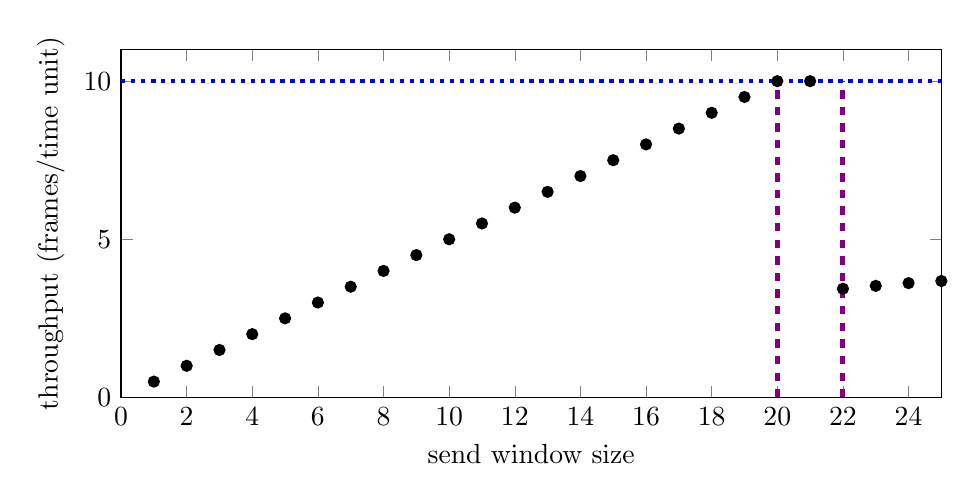
\begin{tikzpicture}
\begin{axis}[width=12cm,height=6cm,
    xlabel=send window size,
    ylabel=throughput (frames/time unit),
    xmin=0,xmax=25,ymin=0]
\addplot[only marks] coordinates {
(1, 0.5000025000125)
(2, 1.0000090000810007)
(3, 1.4999925000374998)
(4, 2.0000280003920055)
(5, 2.500037500562508)
(6, 3.000003000003)
(7, 3.5000035000035)
(8, 4.000048000576006)
(9, 4.499842505512307)
(10, 5.000025000125)
(11, 5.499975250111374)
(12, 5.99977200866367)
(13, 6.499710762871052)
(14, 6.999811005102861)
(15, 7.4996812635462975)
(16, 7.999680012799485)
(17, 8.499426288725509)
(18, 8.999361045365776)
(19, 9.499202067026369)
(20, 9.999100080971061)
(21, 9.999100080973866)
(22, 3.435635094325549)
(23, 3.5274986154570636)
(24, 3.613708966335035)
(25, 3.6808686850100703)
(26, 3.753260645186032)
(27, 3.8487443471573166)
(28, 3.925956461143474)
};
\addplot[blue,dotted,ultra thick,domain=0:25] {10};
    \draw[violet,dashed,ultra thick] (axis cs:20,0) -- (axis cs:20, 10)
     coordinate (empty queue mark);
    \draw[violet,dashed,ultra thick] (axis cs:21.99,0) -- (axis cs:21.99, 10)
     coordinate (full queue mark);
\end{axis}
\end{tikzpicture}
\end{frame}

\begin{frame}[fragile,label=transitTime]{packet transit time}
\begin{tikzpicture}
\draw[ultra thick,arrows={-Latex}] (0, 0) node[left] {sender} -- (1, 0);
\draw[thick] (1, -.5) rectangle (3, .5);
\foreach \x in {2,2.2,2.4,2.6,2.8} {
    \draw (\x, -.5) -- (\x, .5);
}
\node[anchor=south,align=center] at (2, .5) {
    loss when full
};
\node[anchor=north,align=center] at (2, -.5) (queue label) {
    queue
};
\node[anchor=north,font=\fontsize{9}{10}\selectfont] at ([yshift=.3cm]queue label.south) {
    capacity 20
};
\draw[ultra thick,arrows={-Latex}] (3, 0) -- (12, 0) node[right]{receiver}
    node[midway,fill=white,draw=black,very thick,align=left] {
        10 data frames/time unit \\
        1 time unit delay
    }
    node[visible on=<1-3>,ultra thick,pos=0,draw=black,fill=white,font=\tiny,below=.5cm] (data-main) {data};
    \begin{visibleenv}<2->
    \draw[red,-Latex,very thick] (data-main.east) -- (data-main.west -| 13, 0) coordinate (end send)
        node[midway,below,font=\small] {1 time unit (sender to receiver)};
    \end{visibleenv}
\begin{scope}[shift={(12, -4)},x=-1cm]
    \draw[ultra thick,arrows={-Latex}] (0, 0) node[right] {receiver} -- (1, 0);
    \draw[thick] (1, -.5) rectangle (3, .5);
    \foreach \x in {2,2.2,2.4,2.6,2.8} {
        \draw (\x, -.5) -- (\x, .5);
    }
    \node[anchor=south,align=center] at (2, .5) {
        loss when full
    };
    \node[anchor=north,align=center] at (2, -.5) (queue label) {
        queue
    };
    \node[anchor=north,font=\small] at ([yshift=.2cm]queue label.south) {
        capacity 20
    };
    \draw[ultra thick,arrows={-Latex}] (3, 0) -- (12, 0) node[left]{sender}
        node[midway,fill=white,draw=black,very thick,align=left] {
            100 ACK frames/time unit \\
            1 time unit delay
        }
        node[visible on=<2->,pos=0,draw=red,fill=white,font=\tiny,below=.5cm,align=center,inner sep=0.5mm] 
            (ack-start) {a\\c\\k};
    \begin{visibleenv}<2->
        \draw[dotted,red,-Latex,very thick] (end send) |- (ack-start.east);
        \draw[red,-Latex,very thick] (ack-start.west) -- (ack-start.west -| 12, 0) node[midway,below,font=\small] { + 1 time unit (receiver to sender)};
    \end{visibleenv}
\end{scope}
\begin{visibleenv}<3>
\node[draw=red,fill=white,ultra thick,align=left] at (6, -2.5) {
    takes 1 + 1 time units to send message + receive ack \\
    goal: keep sending stuff while waiting
};
\end{visibleenv}
\end{tikzpicture}
\end{frame}

\begin{frame}{filling the pipe}
    \begin{itemize}
    \item round-trip time of 2 time units
        \begin{itemize}
        \item from send data to receive ACK (assuming no queuing delay)
        \end{itemize}
    \item can send 10 data frames per time unit
    \item = can send 20 data frames while waiting for ACK
    \vspace{.5cm}
    \item<2> \myemph{``bandwidth-delay product''}
        \begin{itemize}
        \item 10/time unit (banwidth) times 2 time unit (RTT = delay)
        \end{itemize}
    \end{itemize}
\end{frame}

\begin{frame}[fragile,label=throughAndWindow]{throughput and window size (detail)}
\begin{tikzpicture}
\begin{axis}[width=12cm,height=6cm,
    xlabel=send window size,
    ylabel=throughput (frames/time unit),
    xmin=17,xmax=24,ymin=0]
\addplot[only marks] coordinates {
(1, 0.5000025000125)
(2, 1.0000090000810007)
(3, 1.4999925000374998)
(4, 2.0000280003920055)
(5, 2.500037500562508)
(6, 3.000003000003)
(7, 3.5000035000035)
(8, 4.000048000576006)
(9, 4.499842505512307)
(10, 5.000025000125)
(11, 5.499975250111374)
(12, 5.99977200866367)
(13, 6.499710762871052)
(14, 6.999811005102861)
(15, 7.4996812635462975)
(16, 7.999680012799485)
(17, 8.499426288725509)
(18, 8.999361045365776)
(19, 9.499202067026369)
(20, 9.999100080971061)
(21, 9.999100080973866)
(22, 3.435635094325549)
(23, 3.5274986154570636)
(24, 3.613708966335035)
(25, 3.6808686850100703)
(26, 3.753260645186032)
(27, 3.8487443471573166)
(28, 3.925956461143474)
};
\addplot[blue,dotted,ultra thick,domain=0:25] {10};
    \draw[violet,dashed,ultra thick] (axis cs:20,0) -- (axis cs:20, 11)
     coordinate (empty queue mark);
    \draw[violet,dashed,ultra thick] (axis cs:21.99,0) -- (axis cs:21.99, 11)
     coordinate (full queue mark);
\end{axis}
\node[violet,anchor=south east,align=right] (nq) at ([xshift=1.5cm]empty queue mark) {
    (no queuing delay)
};
\node[violet,anchor=south west,align=left] (mq) at ([xshift=-1.5cm]full queue mark) {
    (max queuing delay)
};
\node[violet,anchor=south] at ($(nq)!0.5!(mq)$) {bandwidth-delay product};
\end{tikzpicture}
\end{frame}


\begin{frame}[fragile,label=fullPipe]{filling the pipe}
\begin{tikzpicture}
\draw[ultra thick,arrows={-Latex}] (0, 0) node[left] {sender} -- (1, 0);
\draw[thick] (1, -.5) rectangle (3, .5);
\foreach \x in {2,2.2,2.4,2.6,2.8} {
    \draw (\x, -.5) -- (\x, .5);
}
\node[anchor=south,align=center] at (2, .5) {
    loss when full
};
\node[anchor=north,align=center] at (2, -.5) (queue label) {
    queue
};
\node[anchor=north,font=\fontsize{9}{10}\selectfont] at ([yshift=.3cm]queue label.south) {
    capacity 20
};
\draw[ultra thick,arrows={-Latex}] (3, 0) -- (12, 0) node[right]{receiver}
    node[midway,fill=white,draw=black,very thick,align=left] {
        10 data frames/time unit \\
        1 time unit delay
    }
    \foreach \x in {0,1,2,3,4,5,6,7,8,9} {
        node[visible on=<3->,pos=\x*.1+0.05,draw=black,fill=white,font=\tiny,below=.5cm] (data-\x) {data}
    };
    \begin{visibleenv}<3->
    \draw[red,Latex-Latex] ([yshift=-.1cm]data-0.south west) -- ([yshift=-.1cm]data-1.south west)
        node[below,font=\small] {0.1 time unit};
    \end{visibleenv}
\begin{scope}[shift={(12, -4)},x=-1cm]
    \draw[ultra thick,arrows={-Latex}] (0, 0) node[right] {receiver} -- (1, 0);
    \draw[thick] (1, -.5) rectangle (3, .5);
    \foreach \x in {2,2.2,2.4,2.6,2.8} {
        \draw (\x, -.5) -- (\x, .5);
    }
    \node[anchor=south,align=center] at (2, .5) {
        loss when full
    };
    \node[anchor=north,align=center] at (2, -.5) (queue label) {
        queue
    };
    \node[anchor=north,font=\small] at ([yshift=.2cm]queue label.south) {
        capacity 20
    };
    \draw[ultra thick,arrows={-Latex}] (3, 0) -- (12, 0) node[left]{sender}
        node[midway,fill=white,draw=black,very thick,align=left] {
            100 ACK frames/time unit \\
            1 time unit delay
        }
        \foreach \x in {0,1,2,3,4,5,6,7,8,9} {
            node[visible on=<3->,pos=\x*.1+0.05,draw=black,fill=white,font=\tiny,below=.5cm,align=center,inner sep=0.5mm] {a\\c\\k}
        };
\end{scope}
\end{tikzpicture}
\end{frame}


\section{why optimal / counting packets in flight}
\begin{frame}{why optimal}
    \begin{itemize}
    \item in normal operation with window size $W$
        \begin{itemize}
        \item receive ACK for $x$ (now $W-1$ in flight)
        \item send packet $x+W$
        \item receive ACK for $x+1$
        \item send packet $x+W+1$
        \item \ldots
        \end{itemize}
    \item window size keeps $W$ packets in flight
    \item if links + queues can hold $W$ packets --- perfect!
    \end{itemize}
\end{frame}

\begin{frame}{number in flight on losses}
    \begin{itemize}
    \item window size $W$
    \item let's say we lose packet $x$ [only], sender might
        \begin{itemize}
        \item receive ACK for $x-1$
        \item send packet $x+W-1$
        \item receive ACK for $x$, $x$, $x$, \ldots
        \item resend packet $x$ (guess it is lost)
        \item \myemph<2>{receive ACK for $x$, $x$, $x$, \ldots}
        \item receive ACK for packet $x+W-1$ 
        \item send packets $x+W$ through $x+W+W-1$
        \end{itemize}
    \end{itemize}
\begin{tikzpicture}[overlay,remember picture]
\begin{visibleenv}<2->
\node[draw=red,ultra thick,anchor=south,align=left] at ([yshift=1cm]current page.south) {
    lots of time where we are not sending packets \\
    means network is underutilized
};
\end{visibleenv}
\end{tikzpicture}
\end{frame}

\begin{frame}{window size tweaking}
    \begin{itemize}
    \item window size imperfect proxy for \# packets in flight
    \item we'll ignore the difference for now
    \vspace{.5cm}
    \item our goal for now: window size = number of packets to have in flight
    \end{itemize}
\end{frame}



\section{searching for performance}
\usetikzlibrary{arrows.meta,shapes.misc,shapes.geometric}
\begin{frame}{finding window size empirically (1)}
\begin{tikzpicture}
\draw[ultra thick,Latex-Latex] (-7, 0) -- (7, 0);
\draw[dotted,line width=2mm,violet] (1, 2) -- (1, -2) node[below] {capacity};
\node[align=left] at (-2, 0) {
    lowest latency \\
    (almost) no losses
};
\node[align=left] at (4.5, 0) {
    highest latency \\
    lots of losses 
};
\end{tikzpicture}
\end{frame}

\begin{frame}{key insight}
    \begin{itemize}
    \item latency/loss rate increases when window size too big
    \item latency/loss rate stable when window size not too big
    \vspace{.5cm}
    \item for now, we'll focus on loss rate
        \begin{itemize}
        \item but you can do something similar with latency
        \end{itemize}
    \end{tiemize}
\end{frame}

\begin{frame}{try a bunch of things}
\begin{tikzpicture}
\tikzset{
    good/.style={draw,star,thick,fill=green!70!black},
    bad/.style={draw,cross out,red!70!black,line width=3mm},
}
\draw[ultra thick,Latex-Latex] (-7, 0) -- (7, 0);
\node at (0, -.5) {window size};
\node[good,label={east:= low loss rate}] (key good) at (-6, 2) {};
\node[bad,label={east:= high loss rate}] (key bad) at (-6, 1) {};
\begin{visibleenv}<2->
\node[good] at (-3, 0){};
\node[bad] (high bad) at (5, 0){};
\end{visibleenv}
\begin{visibleenv}<3->
\node[bad] at (1, 0){}; 
\end{visibleenv}
\begin{visibleenv}<4->
\node[good] at (-1, 0){}; 
\end{visibleenv}
\begin{visibleenv}<5->
\node[good] at (-0.5, 0){}; 
\node[good] at (-0.2, 0){}; 
\node[bad] at (0.3, 0){}; 
\node[bad] at (0.5, 0){}; 
\node[bad] at (0.9, 0){}; 
\end{visibleenv}
\begin{visibleenv}<6>
\draw[Latex-,very thick] (high bad) -- ++(-2, -5) node {
    what is the network like when we do this?
};
\end{visibleenv}
\end{tikzpicture}
\end{frame}


\section{a little history}
\begin{frame}{revisiting congestion collapse}
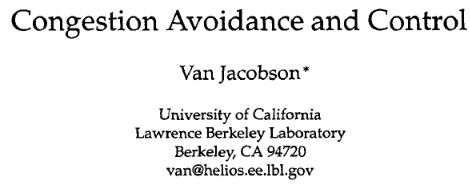
\includegraphics[width=0.6\textwidth]{../congest/jacobson-title}
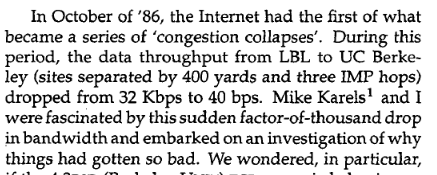
\includegraphics[width=0.6\textwidth]{../congest/jacobson-disaster}
\end{frame}

\begin{frame}<1>[label=jacobsonFixes]{fixes from Jacobson's 1987 paper}
\begin{tikzpicture}
\node[anchor=north west] (fixes) at (0, 0) {
    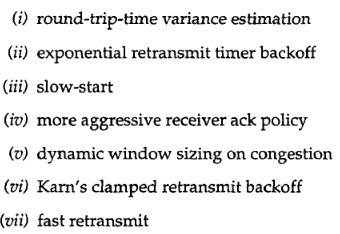
\includegraphics[width=0.6\textwidth]{../congest/jacobson-fixes}
};
%\path[draw,help lines] (0, 0) grid[step=1] (8, -5);
\begin{visibleenv}<2>
    \draw[red,ultra thick] (0, -3.8) rectangle (9, -4.4);
\end{visibleenv}
\begin{visibleenv}<4>
    \draw[red,ultra thick] (0, -2) rectangle (3, -2.8);
\end{visibleenv}
\begin{visibleenv}<3>
    \draw[red,ultra thick] (0, -5.4) rectangle (4.5, -6.2);
\end{visibleenv}
\end{tikzpicture}
\end{frame}


\section{changing cross-traffic}

\usetikzlibrary{arrows.meta,calc,shapes}
\providecommand{\computer}{%
    
\includegraphics[width=1cm]{../common/Noun_project_216.pdf}
}
\providecommand{\switch}{%
    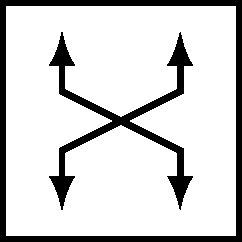
\includegraphics[width=0.9cm]{../common/fig-switch.pdf}
}
\providecommand{\router}{%
    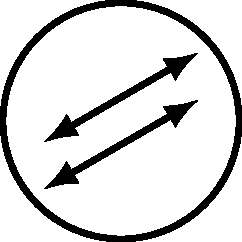
\includegraphics[width=0.9cm]{../common/fig-router.pdf}
}



\begin{frame}{changing cross-traffic}
\begin{tikzpicture}
\tikzset{
    computer/.style={inner sep=0mm,outer sep=0mm,execute at begin node={\computer}},
    switch/.style={inner sep=0mm,outer sep=0mm,execute at begin node={\switch}},
    router/.style={inner sep=0mm,outer sep=0mm,execute at begin node={\router},circle},
    connect/.style={draw,very thick,Latex-Latex},
    connect big/.style={draw,ultra thick,Latex-Latex},
}
\node[computer] (A) at (0, 0){};
\node[computer] (B) at (13, 0){};
\node[router] (r1) at (5, 0){};
\node[router] (r2) at (10, 0){};
\node[computer] (C) at (3, 3){};
\node[computer] (D) at (12, -3){};
\foreach \x/\y in {A/r1,r1/r2,r2/B,C/r1,r2/D} {
    \draw[connect] (\x) -- (\y);
}
\begin{visibleenv}<2>
\foreach \x/\y in {A/r1,r1/r2,r2/B} {
    \draw[blue,line width=1mm] ([yshift=-1mm]\x) -- ([yshift=-1mm]\y);
}
\node[text=blue,anchor=north] at ([yshift=-3mm]$(A)!0.5!(r1)$) {10Mbit};
\end{visibleenv}
\begin{visibleenv}<3>
\foreach \x/\y in {A.east/r1.west,r1.east/r2.west,r2.east/B.west} {
    \draw[-Latex,blue,line width=1mm] ([yshift=-3mm]\x) -- ([yshift=-3mm]\y);
}
\foreach \x/\y in {C/r1,r1.east/r2.west,r2/D} {
    \draw[-Latex,red,dotted,line width=1mm] ([yshift=3mm]\x) -- ([yshift=3mm]\y);
}
\node[text=blue,anchor=north] at ([yshift=-3mm]$(A)!0.5!(r1)$) {\sout{10Mbit} 7Mbit};
\node[text=red,anchor=west] at ($(C)!0.5!(r1)$) {3Mbit};
\end{visibleenv}
\begin{visibleenv}<4>
\foreach \x/\y in {A/r1,r1/r2,r2/B} {
    \draw[blue,line width=1mm] ([yshift=-1mm]\x) -- ([yshift=-1mm]\y);
}
\node[text=blue,anchor=north] at ([yshift=-3mm]$(A)!0.5!(r1)$) {\sout{10Mbit} \sout{7Mbit} 10Mbit};
\end{visibleenv}
\end{tikzpicture}
\end{frame}

\begin{frame}{adapting to cross-traffic}
    \begin{itemize}
    \item available bandwidth will change
    \item previous example: 3Mbit lost/added from other flow
    \vspace{.5cm}
    \item need to adapt to lost bandwidth
    \item need to detect new available bandwidth
    \end{itemize}
\end{frame}

\begin{frame}{other flow's bandwidth?}
    \begin{itemize}
    \item for now, we'll pretend other flows don't react to us
    \vspace{.5cm}
    \item later topic: what happens when both reacting?
    \end{itemize}
\end{frame}


\section{part 1: window sizing}
\againframe<2>{jacobsonFixes}

\section{focus on steady state}
\begin{frame}{handling steady state}
    \begin{itemize}
    \item most of the time we should be at approx. correct window size
    \vspace{.5cm}
    \item want to focus on how we react to changes
    \item still going to use ``experimentation'' idea
    \end{itemize}
\end{frame}


\section{up/down pattern (rough)}
\begin{frame}{window size experimenting}
\begin{tikzpicture}
\tikzset{
    axis line/.style={draw,line width=1mm,-Latex},
    optimum/.style={draw,line width=0.5mm,dashed},
    actual/.style={draw,line width=0.75mm,violet,line to},
    down segment/.style={},
}
    \begin{scope}[y=.8cm,x=.9cm]
        \path[fill=red!10] (0, 6) rectangle (6, 8);
        \path[fill=red!10] (6, 4) rectangle (10, 8);
        \path[fill=red!10] (10, 6) rectangle (14, 8);
        \node[text=red!70!black] at (8, 7) {packets dropped sometimes};
        \node[text=green!70!black] at (8, 2) {packets not dropped};
        
        \path[actual]
            (0, 5.5) to
            (3, 6.3) coordinate (down1) to
            (3, 5.5) to
            (4, 5.8) to
            (6.1, 6.1) coordinate (down2) to
            (6.1, 5.7) to
            (6.5, 5.9) coordinate (down3) to
            (6.5, 5.5) to
            (6.7, 5.7) coordinate (down4) to
            (6.7, 4.8) to
            (6.8, 4.9) coordinate (down5) to
            (6.8, 3.7) to
            (7, 3.8) to
            (8, 4.2) coordinate (down6) to
            (8, 3.5) to
            (9, 3.7) to 
            (10, 4.1) to
            (11, 5.7) to
            (12.5, 6.2) coordinate (down7) to
            (12.5, 5.7) to
            (13, 5.8) to 
            (14, 6.1);

        \foreach \x in {1,...,7} {
            \node[draw=red,cross out,line width=2mm] at (down\x) {};
        };

        \path[axis line] (0, 0) -- (0, 8);
        \path[axis line] (0, 0) -- (14, 0);
        \node[anchor=north] at (7, 0) {time};
        \node[anchor=east,align=center] at (0, 4) {window\\size};
        \path[optimum] (0, 6) -- (6, 6);
        \path[optimum] (6, 4) -- (10, 4);
        \path[optimum] (10, 6) -- (14, 6);
        \begin{visibleenv}<2>
            \node[draw=red,fill=white,ultra thick,align=left,overlay,anchor=north] (up msg) at (3, 2) {
                always try increasing window size
            };
        \end{visibleenv}

        \begin{visibleenv}<3>
            \node[draw=red,fill=white,ultra thick,align=left,overlay,anchor=north] (drop msg) at (3, 2) {
                react to drops \\ by decreasing window
            };
            \foreach \x in {1,...,7} {
                \path[draw=red!50!black, very thick,-Latex] (drop msg) -- (down\x);
            }
        \end{visibleenv}
    \end{scope}
\end{tikzpicture}
\end{frame}

\begin{frame}{increase/decrease strategy}
    \begin{itemize}
    \item default to increasing window size
    \item react to packet drops by decreasing window size
        \begin{itemize}
        \item \myemph<2>{assumption: few ``non-congestion'' packet losses}
        \end{itemize}
    \vspace{.5cm}
    \item<3-> big topic: how fast to do each?
    \item<3-> questions to help decide that:
        \begin{itemize}
        \item what happens if we increase too fast? too slow?
        \item what happens if we decrease too fast? too slow?
        \end{itemize}
    \end{itemize}
\end{frame}

    % FIXME: show sawtooth pattern

\section{performance collapse}
\begin{frame}{the overloaded switch}
\begin{itemize}
\item let's say switch can handle 50 packets/second
\item but has:
    \begin{itemize}
    \item 100 packets/second from test flow sending as fast as it can
    \item 10 packets/second from other session
    \end{itemize}
\item expected \textit{loss rate} (\% packets lost)?
\item expected \% test flow packets lost?
\item expected other session packets lost?
\end{itemize}
\end{frame}

\begin{frame}{modeling who gets dropped}
    \begin{itemize}
    \item it kinda does matter\ldots
    \item sending in big bursts or spread out (``pacing'')?
        \begin{itemize}
        \item bursts can overload queues even though average rate is low
        \end{itemize}
    \item how switch's queue works?
        \begin{itemize}
        \item queue size (handling bursts), way to choose what to drop
        \end{itemize}
    \item random or fixed intervals between sending?
    \vspace{.5cm}
    \item<2-> but we'll \myemph<2>{simplify}, assuming---
        \begin{itemize}
        \item a flow's arrivals are randomly spaced
        \item drops hit packets at random
        \item queue is ``pretty big''
        \end{itemize}
    \end{itemize}
\end{frame}

\begin{frame}{the overloaded switch}
\begin{itemize}
\item let's say switch can handle 50 packets/second
\item but has:
    \begin{itemize}
    \item 100 packets/second from test flow (checking window size) 
    \item 10 packets/second from other session
    \end{itemize}
\item expected \textit{loss rate} (\% packets lost)? $\frac{100+10-50}{100+10}=54\%$
\item expected \% test flow packets lost? $54\%$
\item expected \% other session packets lost? $54\%$
\item<2-> \myemph{\ldots but I missed something}
\end{itemize}
\end{frame}

\begin{frame}{a virtuous cycle}
\begin{itemize}
\item what is other session going to when 54\% of its packets are lost?
    \begin{itemize}
    \item probably resend them
    \end{itemize}
\item what about when resent packets are lost?
    \begin{itemize}
    \item probably resent again
    \end{itemize}
\vspace{.5cm}
\item if other session doesn't slow down, then\ldots
\item $10$ pkt/s $\rightarrow10+54\%\cdot10+54\%^2\cdot10 \ldots\approx 22$ pkt/s
\end{itemize}
\end{frame}


\begin{frame}{the overloaded switch (revised)}
\begin{itemize}
\item let's say switch can handle 50 packets/second
\item but has:
    \begin{itemize}
    \item 100 packets/second from test flow (checking window size) 
    \item 10 packets/second from other session $\rightarrow 22$ with resends
    \end{itemize}
\item expected \textit{loss rate} (\% packets lost)? $\frac{100+22-50}{100+22}=59\%$
\item expected \% test flow packets lost? $59\%$
\item expected \% other session packets lost? $59\%$
    \begin{itemize}
    \item<2-> means that 22 pkt/sec is slight underestimate
    \item<2-> though realistically other session should slow down
    \end{itemize}
\end{itemize}
\end{frame}

\begin{frame}{aside: latency (1)}
\begin{itemize}
\item 589% packet loss $\rightarrow$ average packet sent 2.4 times
\item need one round-trip time (RTT) to detect loss
    \begin{itemize}
    \item probably from duplicate ACK
    \item if detecting via timeout, probably longer
    \end{itemize}
\item so need 1.4 RTTs (detecting loss 1.4 times) extra time 
\item mean latency $= \frac{1.4 \text{RTTs}}{0.5 \text{RTTs}}$ times normal $= 2.8$ times normal
\end{itemize}
\end{frame}

\begin{frame}{aside: high-percentile latency}
\begin{itemize}
\item 59\% packet loss
\item about 10\% of time need more than 4 retransmissions
\item about 5\% of the time need more than 5 retransmissions
\item about 1\% of the time need more than 8 retransmissions
\end{itemize}
\end{frame}

\begin{frame}{sliding windows and retransmissions}
    \begin{itemize}
    \item assuming that other session doesn't slow down
    \vspace{.5cm}
    \item sliding window approach slows down on losses
    \end{itemize}
\end{frame}

\begin{frame}{sliding window throughput collapse}
\begin{itemize}
\item let's say doing sliding window with 100 packet window
\item if 1\% of the time, we need to resend a packet 8 times, then
\item probably need around 8 RTTs to send all 100 packets in window
\vspace{.5cm}
\item<2-> $\approx$ 8 times slower with same window size
\end{itemize}
\end{frame}


\section{heuristic: slow increase}
\begin{frame}{slow increase}
    \begin{itemize}
    \item want to increase \textit{slowly} to avoid overload
    \item original TCP: +1 packet/round trip time
    \vspace{.5cm}
    \item<2-> +1 certainly not optimal choice, but okay heuristic
    \item<2-> important theoretically: approx. \myemph{additive} increase
        \begin{itemize}
        \item helps ensure good behavior with multiple connections
        \item (we'll talk later about why)
        \end{itemize}
    \end{itemize}
\end{frame}


\subsection{exercise: convergence times}
\begin{frame}{exercise: convergence time (1)}
    \begin{itemize}
    \item suppose: 50 ms round trip time
    \item initially sending at 600 packets/second
        \begin{itemize}
        \item $\approx 0.9$Mbyte/sec with 1500 byte packets
        \end{itemize}
    \item optimal rate is 10000 packets/second
        \begin{itemize}
        \item $\approx 15$Mbyte/sec with 1500 byte packets
        \end{itemize}
    \item `standard' TCP increase of 1 packet/RTT
    \item how long to get there?
    \item<2-> current: 30 packets/RTT (= window size 30)
    \item<2-> need to get to: 500 packets/RTT
    \item<2-> will take $500-30=470$ round trips $\approx$ 23500 ms $\approx$ 24 s
    \end{itemize}
\end{frame}

\begin{frame}{fixing bad convergence time}
    \begin{itemize}
    \item TCP's additive increase is very slow for ``high bandwidth-delay'' networks
    \item two things make this better:
    \vspace{.5cm}
    \item not in additive increase mode at start of connection
        \begin{itemize}
        \item ``slow start'' we'll talk about later
        \end{itemize}
    \item more adaptive increase for modern TCP variants
        \begin{itemize}
        \item e.g. FAST TCP, CUBIC TCP, \ldots
        \item heuristics to increase faster when appropriate
        \end{itemize}
    \end{itemize}
\end{frame}


\section{heuristic: fast decrease}
\begin{frame}{fast decrease}
    \begin{itemize}
    \item want to decrease quickly to get out of overload
    \item original TCP heuristic: divide by two (minimum 1 packet)
    \vspace{.5cm}
    \item<2-> exactly by two probably not important
    \item<2-> important theoretically: approx. \myemph{multiplicative} decrease
        \begin{itemize}
        \item will help show okay behavior with multiple flows
        \end{itemize}
    \end{itemize}
\end{frame}

\begin{frame}{AIMD}
    \begin{itemize}
    \item additive increase + multiplicative decrease
    \item basic of steady-state behavior
    \end{itemize}
\end{frame}


% FIXME: decrease on timeout versus dup ACK

\section{some graphs}
\begin{frame}[label=vegasrenotrace]{}
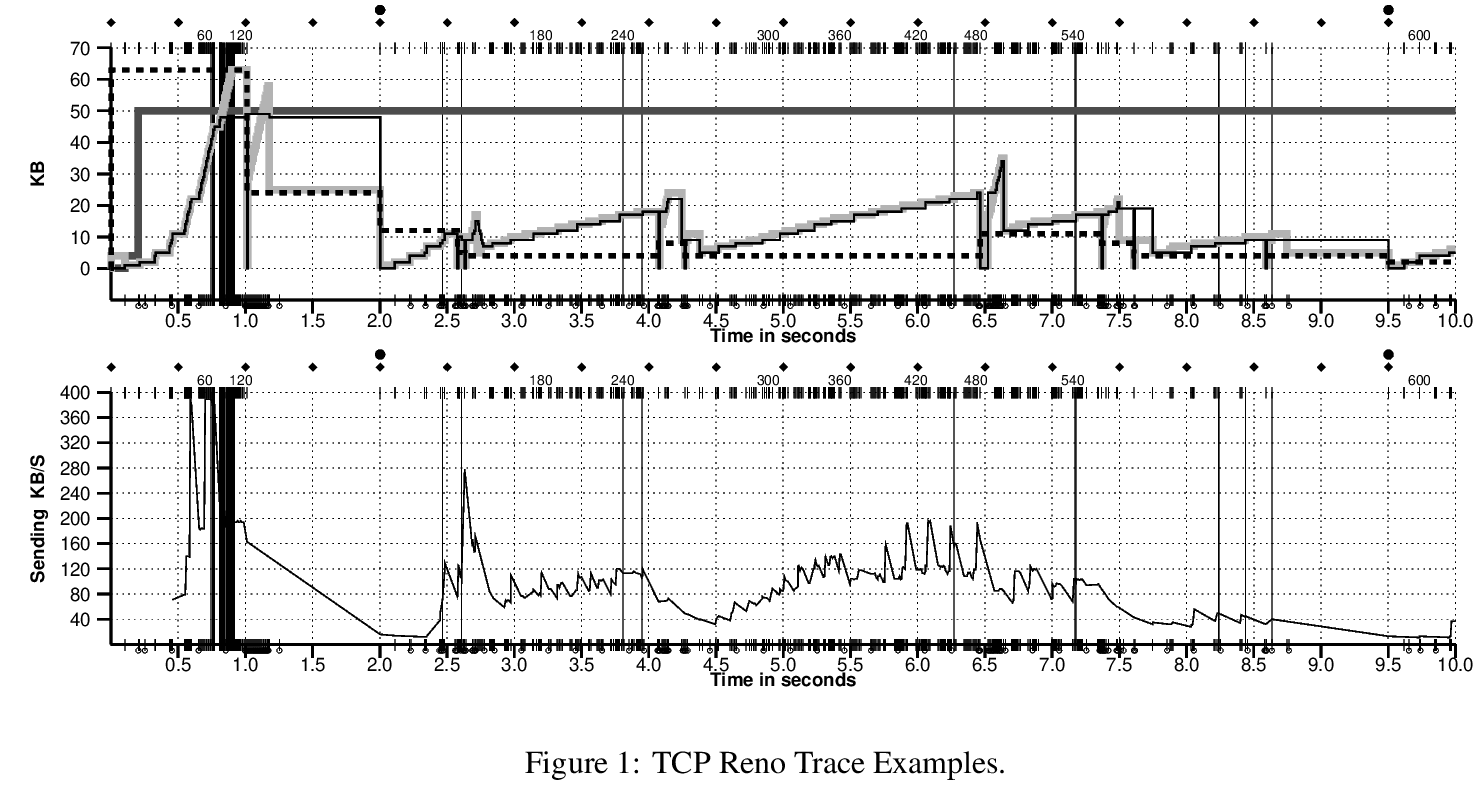
\includegraphics[width=0.9\textwidth]{../congest/vegas-fig1} \\
{
    \tiny from Brakmo, O'Malley, and Peterson, ``TCP Vegas: New techniques for
congestion detection and avoidance''} \\
    \small top thick, light-grey line = congestion window; dotted = slow start threshold
\end{frame}




\section{CUBIC, briefly}
\begin{frame}
\frametitle{CUBIC: default congestion control today}
    \begin{itemize}
    \item default in Linux (since 2006), OS X (since 2014), Windows (since 2019)
        \begin{itemize}
        \item sysadmin has other options they can configure
        \item can be changed on connection-by-connection basis
        \end{itemize}
    \item includes improvements to recovery we'll talk about later
    \item but mostn notably has non-additive increase
    \end{itemize}
\end{frame}

\begin{frame}
    \frametitle{increase intuition}
    \begin{itemize}
        \item `standard' TCP basically has two increase algorithms:
        \item slow start --- quickly explore window sizes
        \item congestion avoidance --- slowly probe for maximum
        \vspace{.5cm}
        \item abrupt transition between these is suspect
            \begin{itemize}
            \item should have gradual exploration $\rightarrow$ fine-tuning switch
            \end{itemize}
        \item heuristic for when to use slow start-style is suspect
            \begin{itemize}
            \item half way from last loss $\approx$ guess?
            \end{itemize}
    \end{itemize}
\end{frame}

\begin{frame}
    \frametitle{CUBIC increase algorithm}
    \begin{itemize}
    \item big idea: faster increase when further away from window size of last loss
        \begin{itemize}
        \item cubic function with saddle point at that window size
        \item function parameterized by time since loss
        \end{itemize}
    \item intuition for `steady state':
        \begin{itemize}
        \item guess correct window size is close to last loss
        \item quickly get to around that window size
        \item search slowly/precisely around that size to fine tune size
        \end{itemize}
    \item intuition for non-steady state:
        \begin{itemize}
        \item try to quickly probe for roughly how small/big it is
        \item worry about getting more precise size on later `pass'
        \end{itemize}
    \end{itemize}
\end{frame}


\begin{frame}{}
\begin{tikzpicture}
\node (pic) {
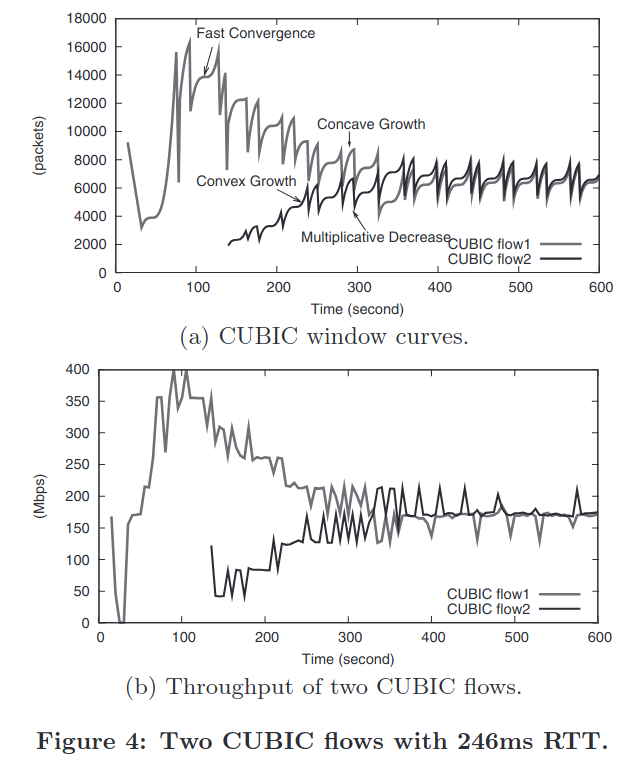
\includegraphics[height=\textheight]{../congest/cubic-fig4}
};
\node[anchor=north west,font=\tiny] at (pic.north east) {
from Ha, Rhee, and Xu, ``CUBIC: A New TCP-Friendly High-Speed TCP Variant''
};
\end{tikzpicture}
\end{frame}

\begin{frame}
    \frametitle{other CUBIC changes}
    \begin{itemize}
        \item different multiplicative decrease factor (divide by 1.4)
    \end{itemize}
\end{frame}


\subsection{exercise: non-congestion losses}
\begin{frame}{non-congestion losses}
    \begin{itemize}
    \item we were ignoring non-congestion losses
    \item suppose \myemph{1\%} loss rate from transmission errors
    \vspace{.5cm}
    \item 100 ms round trip time, very high bandwidth
    \item with TCP heuristics (+1 packet/RTT, half on loss)\ldots
    \item normal window size?
    \end{itemize}
\end{frame}


% FIXME: \subsection{exercise: convergence times}

\section{what about sharing?}
\begin{frame}{congestion: sharing}
    \begin{itemize}
    \item want to consider multiple flows
    \vspace{.5cm}
    \item key questions:
        \begin{itemize}
        \item is it stable if both flows changing window sizes?
        \item is there one winner/loser?
        \item is the winner/loser who we want it to be?
        \end{itemize}
    \end{itemize}
\end{frame}


\subsection{intuition in simple case}
\usetikzlibrary{arrows.meta,calc,shapes}
\providecommand{\computer}{%
    
\includegraphics[width=1cm]{../common/Noun_project_216.pdf}
}
\providecommand{\switch}{%
    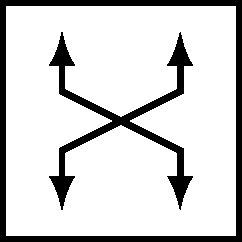
\includegraphics[width=0.9cm]{../common/fig-switch.pdf}
}
\providecommand{\router}{%
    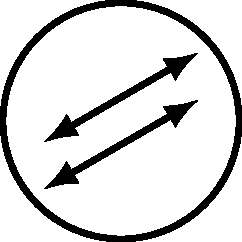
\includegraphics[width=0.9cm]{../common/fig-router.pdf}
}

\begin{frame}{exericse: what should happen?}
\begin{tikzpicture}
\tikzset{
    computer/.style={inner sep=0mm,outer sep=0mm,execute at begin node={\computer}},
    switch/.style={inner sep=0mm,outer sep=0mm,execute at begin node={\switch}},
    router/.style={inner sep=0mm,outer sep=0mm,execute at begin node={\router},circle},
    connect/.style={draw,very thick,Latex-Latex},
    connect big/.style={draw,ultra thick,Latex-Latex},
}
\node[computer] (A) at (0, 0){};
\node[computer] (B) at (13, 0){};
\node[router] (r1) at (5, 0){};
\node[router] (r2) at (10, 0){};
\node[computer] (C) at (3, 3){};
\node[computer] (D) at (12, -3){};
\foreach \x/\y in {A/r1,r1/r2,r2/B,C/r1,r2/D} {
    \draw[connect] (\x) -- (\y);
}
\foreach \x/\y in {A.east/r1.west,r1.east/r2.west,r2.east/B.west} {
    \draw[-Latex,blue,line width=1mm] ([yshift=-3mm]\x) -- ([yshift=-3mm]\y);
}
\foreach \x/\y in {C/r1,r1.east/r2.west,r2/D} {
    \draw[-Latex,red,dotted,line width=1mm] ([yshift=3mm]\x) -- ([yshift=3mm]\y);
}
\end{tikzpicture}
\begin{itemize}
\item two connections on shared link
\item<2-> intuition: each should get half of link bandwidth
\item<3-> question: will this happen if they don't start equal?
\end{itemize}
\end{frame}


\subsection{AIMD convergence}
\usetikzlibrary{arrows.meta,calc,shapes}

\begin{frame}{picturing sharing}
\begin{tikzpicture}
\tikzset{
    axis/.style={
        draw,ultra thick,-Latex
    },
    normal mark/.style={
        fill=black,
        alt=<5->{fill=black!50},
    },
    normal adjust/.style={
        line width=.5mm,draw=black!50!red,-Latex,
        alt=<5->{draw=black!50!red!50},
    },
}
\begin{scope}[x=1.2cm,y=1.2cm] 
    \path[fill=red!10] (5.5, 0) -- (5.0, 0) -- (0, 5) -- (0, 5.5) -- (5.5, 5.5) -- cycle;
    \path[axis] (0, 0) -- (5.5, 0)
        node[midway,below] {flow 1 bandwidth};
    \path[axis] (0, 0) -- (0, 5.5)
        node[midway,left,align=right] {flow 2\\bandwidth};
    \path[draw,dashed,very thick] (5, 0) -- (0, 5);
    \node[text=red,visible on=<1-3>] at (4, 4) {
        overloaded
    };
    \node[text=black,visible on=<1-3>] at (1.5, 2) {
        underloaded
    };

    \begin{visibleenv}<2>
        \path[draw=black!50,dotted, very thick] (4.5 * 1.2, 2 * 1.2) -- (0, 0);
        \path[line width=1mm,draw=black!50!red,-Latex] (4.5, 2) -- (2.25 * 1.07, 1 * 1.07);
        \path[fill=black] (4.5, 2) circle (2mm);
        \path[fill=black!50] (2.25, 1) circle (2mm);
        \node[anchor=north west,align=left] (incr box) at (4, 4) {
            multiplicative decrease \\
            moves bandwidths along line to origin \\
            example: (90\%, 40\%) to (45\%, 20\%)
        };
        %\draw[violet,very thick] (incr box) -- (4.5, 2+2mm);
    \end{visibleenv}

    \begin{visibleenv}<3>
        \path[draw=black!50,dotted, very thick] (2.25 - 1, 1 - 1) -- (5.5, 1 + 5.5 - 2.25);
        \path[fill=black] (2.25, 1) circle (2mm);
        \path[fill=black!50] (2.25 + 1.3, 1 + 1.3) circle (2mm);
        \node[anchor=north west,align=left] (decr box) at (4, 3) {
            additive decrease \\
            moves bandwidths \\
            at 45-degree angle \\
            example: (45\%, 20\%) to (55\%, 30\%)
        };
    \end{visibleenv}

    \begin{visibleenv}<4->
        \path[normal adjust] (4.5, 2) -- (2.25 * 1.07, 1 * 1.07);
        \path[normal adjust] (2.25 + .14, 1 + .14) -- (2.25 + 1.3 -.14, 1 + 1.3 -.14);
        \path[normal adjust] (2.25 + 1.3 -.14, 1 + 1.3 -.14) -- (1.775*1.07, 1.15*1.07);
        \path[normal adjust] (1.775*1.07, 1.15*1.07) -- (1.775 + 1.3 -.14, 1.15 + 1.3 -.14);
        \path[normal adjust] (1.775 + 1.3 -.14, 1.15 + 1.3 -.14)
            -- (1.5375 * 1.07, 1.225 * 1.07);
        \path[normal adjust] (1.5375 * 1.07, 1.225 * 1.07)
            -- (1.5375 + 1.4 - .14, 1.225 + 1.4 - .14);
        \path[normal adjust] (1.5375 + 1.4 - .14, 1.225 + 1.4 - .14)
            -- (1.4687 * 1.07, 1.325 * 1.07);
        \path[normal mark] (4.5, 2) circle (2mm);
        \path[normal mark] (2.25, 1) circle (2mm);
        \path[normal mark] (2.25 + 1.3, 1 + 1.3) circle (2mm);
        \path[normal mark] (1.775, 1.15) circle (2mm);
        \path[normal mark] (1.775 + 1.3, 1.15 + 1.3) circle (2mm);
        \path[normal mark] (1.5375, 1.225) circle (2mm);
        \path[normal mark] (1.5375 + 1.4, 1.225 + 1.4) circle (2mm);
        \path[normal mark] (1.4687, 1.325) circle (2mm);
    \end{visibleenv}

    \begin{visibleenv}<5->
        \path[draw=black,dashed,very thick] (0,0) -- (5.5, 5.5)
            node[pos=0.75,sloped,above] {equal bandwidth};
    \end{visibleenv}
    \begin{visibleenv}<6>
        \node[anchor=north west,align=left] at (5, 4) {
            multiplicative decrease brings \\
            closer to equal bandwidth line \\
            ~ \\
            additive increase keeps same \\
            distance from line
        };
    \end{visibleenv}
\end{scope}
\end{tikzpicture}
\end{frame}


\subsection{when one host can't saturate link}
% FIXME: show diagram where one host constrained by other link
\usetikzlibrary{arrows.meta,calc,shapes,decorations.pathreplacing,patterns}
\providecommand{\computer}{%
    
\includegraphics[width=1cm]{../common/Noun_project_216.pdf}
}
\providecommand{\switch}{%
    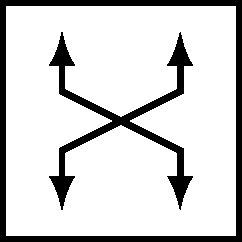
\includegraphics[width=0.9cm]{../common/fig-switch.pdf}
}
\providecommand{\router}{%
    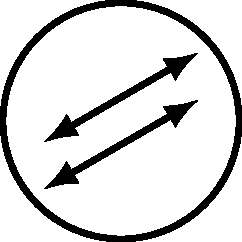
\includegraphics[width=0.9cm]{../common/fig-router.pdf}
}



\begin{frame}{a scenario}
\begin{tikzpicture}
\tikzset{
    computer/.style={inner sep=0mm,outer sep=0mm,execute at begin node={\computer}},
    switch/.style={inner sep=0mm,outer sep=0mm,execute at begin node={\switch}},
    router/.style={inner sep=-1mm,outer sep=0mm,execute at begin node={\router},circle},
    connect/.style={draw,line width=0.5mm,Latex-Latex},
    connect big/.style={draw,line width=1mm,Latex-Latex},
}
\node[computer] (A) at (0, 2){};
\node[computer] (B) at (13, 0){};
\node[router] (r1) at (5, 0){};
\node[router] (r2) at (10, 0){};
\node[computer] (C) at (0, -2){};
\node[computer] (D) at (13, -2){};
\foreach \x/\y in {A/r1,r1/r2,r2/B,r2/D} {
    \draw[connect big] (\x) -- (\y);
}
\draw[connect] (C) -- (r1)
    node[midway,pin={slow link}] {};
\begin{visibleenv}<2>
\foreach \x/\y in {A.east/r1.west,r1.east/r2.west,r2.east/B.west} {
    \draw[-Latex,blue,line width=.7mm] ([yshift=-3mm]\x) -- ([yshift=-3mm]\y);
}
\foreach \x/\y in {C.north east/r1.south west,r1.east/r2.west,r2/D} {
    \draw[-Latex,red,dotted,line width=.5mm] ([yshift=3mm]\x) -- ([yshift=3mm]\y);
}
\end{visibleenv}
\end{tikzpicture}
\end{frame}

\begin{frame}{slow link + mixed traffic}
\begin{tikzpicture}
\tikzset{
    axis/.style={
        draw,ultra thick,-Latex
    },
    normal mark/.style={
        fill=black,
    },
    normal adjust/.style={
        line width=.5mm,draw=black!50!red,-Latex,
    },
}
\begin{scope}[x=1.2cm,y=1.2cm] 
    \path[pattern=checkerboard,pattern color=red!10] (0, 5) -- (3.5, 1.5) -- (0, 1.5) -- cycle;
    \path[fill=red!10,alt=<3>{draw=red,line width=4mm}] (5.5, 0) -- (5.0, 0) -- (0, 5) -- (0, 5.5) -- (5.5, 5.5) -- cycle;
    \begin{visibleenv}<4>
        \path[draw=red,line width=4mm] (0, 5) -- (3.5, 1.5) -- (0, 1.5) -- cycle;
    \end{visibleenv}
    \begin{visibleenv}<5>
        \path[draw=red,line width=4mm] (0, 0) -- (0, 1.5) -- (3.5, 1.5) -- (5, 0) -- cycle;
    \end{visibleenv}
    \path[axis] (0, 0) -- (5.5, 0)
        node[midway,below] {flow 1 bandwidth};
    \path[axis] (0, 0) -- (0, 5.5)
        node[midway,left,align=right] {flow 2\\bandwidth};
    \path[draw,dashed,very thick,alt=<2>{red,very thick}] (5, 0) -- (0, 5);
    \draw[draw,dashed,very thick,alt=<2>{red,very thick}] (0, 1.5) -- (3.5, 1.5);
    \node[text=red] at (3.5, 4) {both flows get drops};
    \node[text=red,align=center] at (1.3, 2.5) {flow 2 \\ gets drops};

    \begin{visibleenv}<2>
         \path[draw,violet,ultra thick,Latex-] (3, 2) -- ++(1, 1) coordinate (fast link msg) node[right] {
             limit of fast link's bandwidth
         };
         \path[draw,violet,ultra thick,Latex-] (2, 3) -- (fast link msg);
         \path[draw,violet,ultra thick,Latex-] (1, 4) -- (fast link msg);
         \path[draw,violet,ultra thick,Latex-] (3.8, 1.2) -- (fast link msg);
         \path[draw,violet,ultra thick,Latex-] (3.3, 1.45) -- ++(1.5, -1) coordinate (slow link msg) node[right] {
             limit of slow link's bandwidth
         };
         \path[draw,violet,ultra thick,Latex-] (2.3, 1.45) -- (slow link msg);
         \path[draw,violet,ultra thick,Latex-] (1.3, 1.45) -- (slow link msg);
    \end{visibleenv}
    
    \begin{visibleenv}<3->
        \begin{scope}[alt=<4->{opacity=0.5}]
        \path[normal adjust] (4, 3) -- ++(-1, -0.75);
        \path[normal adjust] (5, 3) -- ++(-1.25, -0.75);
        \path[normal adjust] (5, 2) -- ++(-1.25, -0.5);
        \path[fill=black] (5, 3) circle (2mm);
        \path[fill=black] (4, 3) circle (2mm);
        \path[fill=black] (5, 2) circle (2mm);
        \end{scope}
    \end{visibleenv}
    \begin{visibleenv}<3>
        \node[anchor=west,align=left] at (6, 3) {
            if both flows see drops, \\
            multiplicative decrease \\
            (toward origin)
        };
    \end{visibleenv}

    \begin{visibleenv}<4->
        \begin{scope}[alt=<5->{opacity=0.5}]
        \path[normal adjust] (1, 3) -- ++(0.8,-1.1);
        \path[normal adjust] (2, 2.8) -- ++(0.8,-1.4);
        \path[normal adjust] (2, 2) -- ++(0.8,-1.1);
        \path[fill=black] (1, 3) circle (2mm);
        \path[fill=black] (2, 2.8) circle (2mm);
        \path[fill=black] (2, 2) circle (2mm);
        \end{scope}
    \end{visibleenv}
    \begin{visibleenv}<4>
        \node[anchor=west,align=left] at (6, 3) {
            if only flow 2 see drops, \\
            it decreases bandwidth and \\
            flow 1 increase bandwidth

        };
    \end{visibleenv}
    \begin{visibleenv}<5->
        \begin{scope}[alt=<6->{opacity=0.5}]
        \path[normal adjust] (1, 1) -- ++(0.8, .8);
        \path[normal adjust] (1, 0.5) -- ++(0.8, 0.8);
        \path[normal adjust] (2, 0.25) -- ++(0.8, 0.8);
        \path[normal adjust] (4, 0.25) -- ++(0.8, 0.8);
        \path[fill=black] (1, 1) circle (2mm);
        \path[fill=black] (1, 0.5) circle (2mm);
        \path[fill=black] (2, 0.25) circle (2mm);
        \path[fill=black] (4, 0.25) circle (2mm);
        \end{scope}
    \end{visibleenv}
    \begin{visibleenv}<5>
        \node[anchor=west,align=left] at (6, 3) {
            if both flows see no drops, \\
            both increase additively  \\
            (45 degree angle)
        };
    \end{visibleenv}
    \begin{visibleenv}<6>
        \path[fill=red] (3.5, 1.5) circle (4mm);
        \path[fill=black] (3.5, 1.5) circle (2mm);
        \node[anchor=west,align=left] at (6, 3) {
            result: flow 2 reaches \\
            limit of slow link \\
            flow 1 gets the rest \\
            of the bandwidth
        };
    \end{visibleenv}
\end{scope}
\end{tikzpicture}
\end{frame}


\subsection{min/max fairness}
\begin{frame}{fairness metrics}
    \begin{itemize}
    \item would like to say both allocations are `fair'
    \item not equal, but most equal we can give on network
    \vspace{.5cm}
    \item would like some way of formalizing this
    \end{itemize}
\end{frame}

\begin{frame}{fairness intuition}
    \begin{itemize}
    \item unfair allocation = someone gets much less than others
    \vspace{.5cm}
    \item consequence: let's look for ``starved'' flow
    \item if we can add to starved flow\ldots \\
          without hurting more starved flows\ldots \\
          then that's ``unfair''
    \end{itemize}
\end{frame}


\subsubsection{exercise}

\usetikzlibrary{arrows.meta,calc,shapes,decorations.pathreplacing,patterns}
\providecommand{\computer}{%
    
\includegraphics[width=1cm]{../common/Noun_project_216.pdf}
}
\providecommand{\switch}{%
    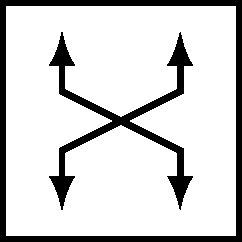
\includegraphics[width=0.9cm]{../common/fig-switch.pdf}
}
\providecommand{\router}{%
    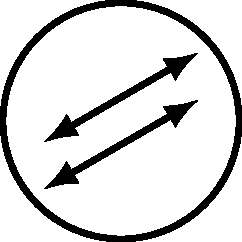
\includegraphics[width=0.9cm]{../common/fig-router.pdf}
}



\begin{frame}{exercise}
\begin{tikzpicture}
\tikzset{
    computer/.style={inner sep=0mm,outer sep=0mm,execute at begin node={\computer}},
    switch/.style={inner sep=0mm,outer sep=0mm,execute at begin node={\switch}},
    router/.style={inner sep=-1mm,outer sep=0mm,execute at begin node={\router},circle},
    connect/.style={draw,line width=0.5mm,Latex-Latex},
    connect big/.style={draw,line width=1mm,Latex-Latex},
}
\node[computer] (A) at (0, 2){};
\node[computer] (B) at (13, 0){};
\node[router] (r1) at (5, 0){};
\node[router] (r2) at (10, 0){};
\node[computer] (C) at (0, -2){};
\node[computer] (D) at (13, -2){};
\foreach \x/\y in {A/r1,r1/r2,r2/B,r2/D} {
    \draw[connect big] (\x) -- (\y);
}
\draw[connect] (C) -- (r1)
    node[midway,every pin/.style={arrows=-},pin={slow link}] {};
\begin{visibleenv}<2>
\foreach \x/\y in {A.east/r1.west,r1.east/r2.west,r2.east/B.west} {
    \draw[-Latex,blue,line width=.7mm] ([yshift=-3mm]\x) -- ([yshift=-3mm]\y);
}
\foreach \x/\y in {C.north east/r1.south west,r1.east/r2.west,r2/D} {
    \draw[-Latex,red,dotted,line width=.5mm] ([yshift=3mm]\x) -- ([yshift=3mm]\y);
    \draw[-Latex,violet,dashed,line width=.5mm] ([yshift=5mm]\x) -- ([yshift=5mm]\y);
}
\end{visibleenv}
\end{tikzpicture}
\begin{itemize}
\item let's say slow link has 5 MByte/s capacity, other links 20MByte/s
\item why are these fair/unfair? (by min-max fairness)
    \begin{itemize}
    \item solid = 10MByte, dotted = 2MByte/s, dashed = 3MByte/s
    \item solid = 16MByte, dashed = 2MByte/s, dashed = 2MByte/s
    \end{itemize}
\end{itemize}
\end{frame}



\subsection{Jain's fairness index}
\begin{frame}{Jain's fairness index}
    \begin{itemize}
    \item more common metric, but for scenarios where equal allocation makes sense
    \vspace{.5cm}
    \item if $x_i$ is i'th flow's share: \\
    \[\frac{\left(\sum x_i\right)^2}{n\cdot\sum x_i^2}\]
    \vspace{.5cm}
    \item approaches 1 when allocations equal, $\frac{1}{n}$ if one flow gets everything
    \end{itemize}
\end{frame}


\subsection{RTT-unfairness}
\begin{frame}{long links}
\begin{tikzpicture}
\tikzset{
    computer/.style={inner sep=0mm,outer sep=0mm,execute at begin node={\computer}},
    switch/.style={inner sep=0mm,outer sep=0mm,execute at begin node={\switch}},
    router/.style={inner sep=-1mm,outer sep=0mm,execute at begin node={\router},circle},
    connect/.style={draw,line width=0.5mm,Latex-Latex},
    connect big/.style={draw,line width=1mm,Latex-Latex},
}
\node[computer] (A) at (0, 2){};
\node[computer] (B) at (13, 0){};
\node[router] (r1) at (5, 0){};
\node[router] (r2) at (10, 0){};
\node[computer] (C) at (-1, -4){};
\node[computer] (D) at (12, -2){};
\foreach \x/\y in {A/r1,r1/r2,r2/B,r2/D} {
    \draw[connect big] (\x) -- (\y);
}
\draw[connect big] (C) -- (r1)
    node[-,sloped,midway,pin={long link},every pin edge/.style={-}] {};
\begin{visibleenv}<2>
\foreach \x/\y in {A.east/r1.west,r1.east/r2.west,r2.east/B.west} {
    \draw[-Latex,blue,line width=.7mm] ([yshift=-3mm]\x) -- ([yshift=-3mm]\y);
}
\foreach \x/\y in {C.north east/r1.south west,r1.east/r2.west,r2/D} {
    \draw[-Latex,red,dotted,line width=.7mm] ([yshift=3mm]\x) -- ([yshift=3mm]\y);
}
\end{visibleenv}
\end{tikzpicture}
\end{frame}

\begin{frame}{exercise: window size?}
    \begin{itemize}
    \item flow 1: 500 packets/sec, 50 ms round trip
    \item flow 2: 500 packets/sec, 100 ms round trip
    \vspace{.5cm}
    \item exercise: what window size achieves this for each flow?
        \begin{itemize}
        \item<2-> 1: window size 25; 2: window size 50
        \end{itemize}
    \end{itemize}
\end{frame}

\begin{frame}{revisiting additive increase}
    \begin{itemize}
    \item TCP: add +1 to window size each round trip time
    \item flow 1: window 25+1 $\rightarrow$ 26 pkt/50 ms = 520 pkt/sec
    \item flow 2: window 50+1 $\rightarrow$ 51 pkt/100 ms = 510 pkt/sec
    \end{itemize}
\begin{tikzpicture}
\tikzset{
    axis/.style={
        draw,ultra thick,-Latex
    },
    normal mark/.style={
        fill=black,
    },
    normal adjust/.style={
        line width=.5mm,draw=black!50!red,-Latex,
    },
}
\begin{scope}[x=.8cm,y=.8cm] 
    \path[fill=red!10] (5.5, 0) -- (5.0, 0) -- (0, 5) -- (0, 5.5) -- (5.5, 5.5) -- cycle;
    \path[axis] (0, 0) -- (5.5, 0)
        node[midway,below] {flow 1 bandwidth};
    \path[axis] (0, 0) -- (0, 5.5)
        node[midway,left,align=right] {flow 2\\bandwidth};
    \path[draw,dashed,very thick] (5, 0) -- (0, 5);

    \begin{visibleenv}<2>
        \path[draw,dotted,very thick] (0, 0) -- (3.333 * 1.5, 1.667 * 1.5);
        \path[draw,dotted,very thick] (2, 2) -- ++(3.333 * 1, 1.667 * 1);
        \path[draw,dotted,very thick] (2, 2) -- ++(-3.333 * 0.7, -1.667 * 0.7);
    \end{visibleenv}

    \path[normal adjust] (2, 2) -- ++(1, .5);
    \path[normal mark] (2, 2) circle (1mm);
    \path[dotted,-Latex,line width=.5mm,draw=black!50] (2,2) -- ++ (1, 1);
    \begin{visibleenv}<1>
    \node[align=left,anchor=west] at (6, 2.5) {
        flow 1 increases faster \\
        than flow 2 increases \\
        not 45-degree angle anymore
    };
    \end{visibleenv}
    \begin{visibleenv}<2>
        \path[fill=red] (3.333, 1.667) circle (2mm);
        \path[fill=black] (3.333, 1.667) circle (1mm);
        \node[align=left,anchor=west] at (6, 2.5) {
            in equilibrium \\
            flow 1 gets more bandwidth
        };
        \end{visibleenv}
\end{scope}
\end{tikzpicture}
\end{frame}


\subsection{other unfairness}
\begin{frame}{other unfairness}
    \begin{itemize}
    \item lower round-trip gets more bandwidth
    \item can also get more bandwidth by\ldots
    \vspace{.5cm}
    \item using more connections (`independent' windows)
    \item adding more than + 1 packet to window size/RTT
    \end{itemize}
\end{frame}

\begin{frame}{alternate congestion control}
    \begin{itemize}
    \item usually \textit{more aggressive} than ``normal'' TCP
        \begin{itemize}
        \item examples we'll talk about later: CUBIC, Compound TCP \\
            (common defaults on recentish OSes)
        \item needed to fully utilize bandwidth on fast network
        \end{itemize}
    \vspace{.5cm}
    \item concern: are these ``stealing'' all the bandwidth from normal TCP?
    \item ``TCP-friendly''
        \begin{itemize}
        \item should not make TCP used alongside them behave poorly
        \end{itemize}
    \end{itemize}
\end{frame}

\begin{frame}{examples: TCP-unfriendliness}
\begin{tikzpicture}
\node (a) {
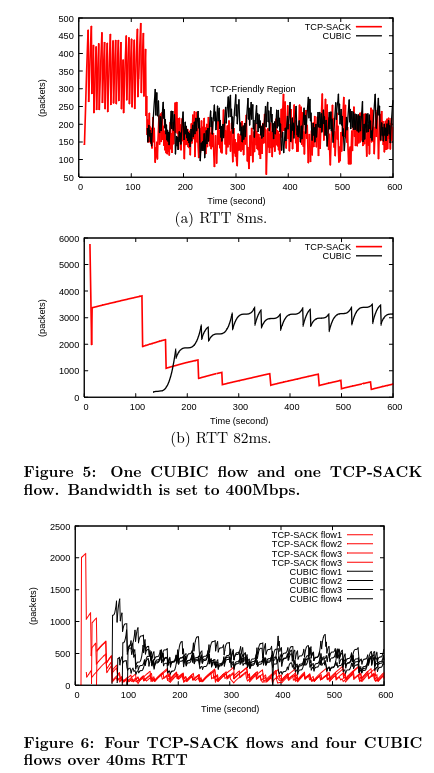
\includegraphics[height=0.9\textheight]{../congest/cubic-sack-compare}
};
\node[anchor=north west] (b) at (a.north east) {
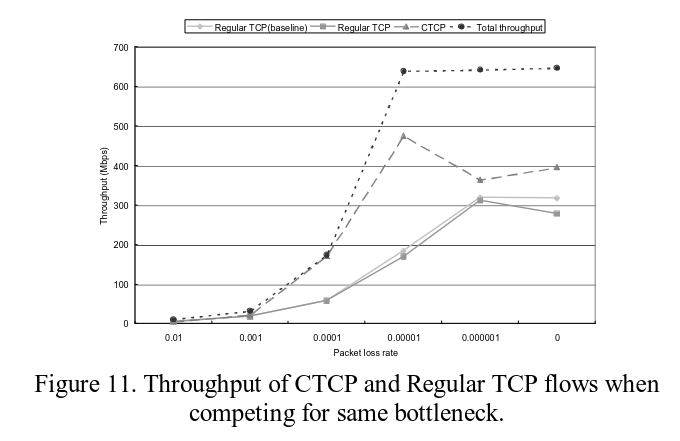
\includegraphics[height=0.6\textheight]{../congest/ctcp-regular-compare}
};
\end{tikzpicture}
\imagecredit{
from Ha, et al, ``CUBIC: A New TCP-Friendly High-Speed TCP Variant'' \\
and Tan, et al, ``A Compound TCP Approach for High-speed and Long Distance Networks''
}
\end{frame}


\subsubsection{unfairness in practice}
\begin{frame}{a theoretical result}
    \begin{itemize}
    \item for RTT-unfairness, standard TCP with selective acknowledgments:\footnote{Mathis et al, ``The Macroscopeic Behavior of the TCP Congestion Avoidance Algorithm'' (1997)}
    \[\text{throughput} \approx \text{constant} \times \frac{\text{packet size}}{\text{RTT}\sqrt{\text{loss rate}}}\]
    \end{itemize}
\end{frame}

\begin{frame}{empirical results}
    \begin{itemize}
    \item some results from Philip (IMC'21)\footnote{Philip, Ware, Athapathu, Sherry, Sekar, ``Revisting TCP Congestion Control Throughput Models \& Fairness Properties At Scale'' (IMC'21)}
    \item with same congestion control algorithm + RTT, Jain's fairness index > 0.99
    \item CUBIC takes 70-80\% of throughput when competing with equal number of traditional TCP flows
        \begin{itemize}
        \item recall: major change is cubic increase curve instead of additive (linear) increase
        \end{itemize}
    \end{itemize}
\end{frame}


\section{`fast retransmit' and `fast recovery'}
\againframe<3>{jacobsonFixes}

\subsection{recall: duplicate ACKs}
\begin{frame}{fast retransmit}
    \begin{itemize}
    \item if large window + data packet 2 is lost, then sender will see
    \item ACK 0, \myemph{ACK 1, ACK 1, ACK 1, ACK 1, ACK 1}
    \item duplicate ACKs indicate missing packet 2
    \item \myemph{shouldn't wait for timeout}
    \vspace{.5cm}
    \item<2-> $\rightarrow$ TCP heuristic: retransmit immediately after $\sim$3 duplicate ACKs
        \begin{itemize}
        \item not 1 duplicate ACK to tolerate some reordering
        \item also some other details (we'll talk later)
        \end{itemize}
    \end{itemize}
\end{frame}



\subsection{duplicate ACKs}
\begin{frame}{fast retransmission}
    \begin{itemize}
    \item TCP calls this idea of retransmission from duplicate ACKs  \\
        ``fast retransmission''
        \begin{itemize}
        \item was actually not done in early versions of TCP
        \end{itemize}
    \vspace{.5cm}
    \item but problem: what to do with congestion window
    \item solution called `fast recovery'
    \end{itemize}
\end{frame}
 % FIXME: missing from elsewhere

\subsection{intuition: self-clocking}
\begin{frame}{self-clocking and dup-ACKs}
    \begin{itemize}
    \item without losses, sender sends one new packet per ACK
    \item keeps number of packets in network constant
    \item but duplicate ACKs are exception (say window size 6):
    \end{itemize}
{\fontsize{10}{11}\selectfont
\begin{tabular}{llll}
recv'd & sent & count of packets in flight \\ \hline
--- & data 0-5 & 6 \\
ACK 0 & ~ & 5 \\
~ & data 6 & 6 \\
ACK 1 & ~ & 5 \\
~ & data 7 & 6 \\
ACK 1 & ~  & 5 \\
ACK 1 & ~  & 4 \\
ACK 1 & ~ & 3 \\
~ & data 2 & 4 \\
ACK 1 & ~ & 3 \\
\end{tabular}
}
\end{frame}

\begin{frame}{alternate explanation}
    \begin{itemize}
    \item sender stopped sending while receiving duplicate ACKs
    \item but we know \textit{most messages got there}
    \item means our usage of network doesn't reflect out window size
    \end{itemize}
\end{frame}

\begin{frame}{TCP's fast retransmission}
\begin{itemize}
\item on third duplicate ACK:
\vspace{.5cm}
\item resend packet,
\item do multiplicative decrease, AND THEN
\item temporarily add 2 packet to window for each dup ACK
    \begin{itemize}
    \item send packets to replace received packet
    \item (if allowed by multiplicative-decreased window)
    \end{itemize}
\item reset window size back when later ACK
\end{itemize}
\end{frame}

\begin{frame}{self-clocking and fast retransmit}
\begin{itemize}
\item adjust window size to keep packets in flight constant:
\end{itemize}
{\fontsize{9}{10}\selectfont
\begin{tabular}{llll}
recv'd & sent & count packets in flight & send window size (range) \\ \hline
--- & data 0-5 & 6 & 6 (0-5)\\
ACK 0 & ~ & 5 & 6 (1-6) \\
~ & data 6 & 6 & 6 (1-6)\\
ACK 1 & ~ & 5 & 6 (2-7)\\
~ & data 7 & 6 & 6 (2-7)\\
ACK 1 & ~  & 5 & 6 (2-7)\\
ACK 1 & ~  & 4 & 6 (2-7)\\
ACK 1 & ~ & 3 & 6 (2-7) \\
~ & data 2 & 4 & \myemph{8} (2-9)\\
~ & \myemph{data 8} & 5 & 8 (2-9)\\
~ & \myemph{data 9} & 6 & 8 (2-9)\\
ACK 1 & ~ & 5 & \myemph{9} (2-10)  \\
~ 1 & \myemph{data 10} & 5 & \myemph{9} (2-10)  \\
\end{tabular}
}
\end{frame}


% FIXME: watching latency

%\section{slow start later}

\begin{frame}{``slow start'' later}
    % FIXME: diagram
    \begin{itemize}
    \item heuristic: slow start if window size is `small' compared to last packet loss
        \begin{itemize}
        \item compromise: find correct size v. overload network
        \end{itemize}
    \vspace{.5cm}
    \item method:
    \item set \texttt{ssthresh} = bytes in flight / 2 on packet loss
    \item use slow start when window size < \texttt{ssthresh}
    \end{itemize}
\end{frame}



\end{document}
